\documentclass[12pt,letterpaper]{article}
\usepackage[margin=1.5in]{geometry}
\usepackage[spanish,es-nodecimaldot]{babel}
\newcommand\hmmax{0}
\newcommand\bmmax{0}
\usepackage[utf8]{inputenc}
\usepackage[T1]{fontenc}
\usepackage{eurosym}
\usepackage{charter,mathpazo}
\usepackage{amsmath,amssymb}
\usepackage{amsfonts}
\usepackage{units}
\usepackage{graphicx}
\usepackage{tabularx}
\usepackage{subfig}
\usepackage{kpfonts}
\usepackage{microtype}
\usepackage{booktabs}
\usepackage{bm}
\usepackage{listings}
\usepackage{verbatim}
\usepackage{color,soul}
\usepackage[colorlinks=false]{hyperref}
\usepackage{natbib}
\usepackage{eurosym}
\newcommand{\e}{\mathrm{e}}

\begin{document}
\title{\textbf{Incentivos y estructura organizativa en la financiaci\'on hospitalaria}\\{\small \textbf{}}}
\author{Jose Mar\'\i a Elena-Izquierdo}
\date{}
\maketitle

\begin{abstract}
La financiaci\'on hospitalaria eficiente depende de los arreglos organizativos establecidos entre los distintos agentes que interact\'uan. En este trabajo estudiamos c\'omo, bajo riesgo moral, diferentes estructuras organizativas moldean el papel de los mecanismos de pago por incentivos para los m\'edicos y los directivos hospitalarios. Utilizando un modelo de m\'ultiples tareas con dos niveles, caracterizamos la soluci\'on de segundo \emph{best} bajo contrataci\'on centralizada y descentralizada. Mediante simulaciones num\'ericas, mostramos c\'omo las variaciones en el ruido de las se\~nales y en el grado de complementariedad o sustituibilidad entre tareas afectan a la potencia \^optima de los incentivos, as\'i como a los niveles de esfuerzo de los agentes.
\end{abstract}

\section*{Introducci\'on}
La provisi\'on de servicios hospitalarios de atenci\'on sanitaria es, en \`ultima instancia, el resultado de la interacci\'on de m\'ultiples agentes. Por un lado, los financiadores (p\'ublicos o privados) compran esos servicios a los hospitales. Los gestores, por otro lado, toman continuamente decisiones sobre la asignaci\'on de recursos humanos y materiales. Junto con ello, dentro de un hospital hay una multiplicidad de agentes con tareas distintas a su cargo: m\'edicos, personal de enfermer\'ia, auxiliares, farmac\'euticos, etc. Las acciones y esfuerzos combinados de todos estos agentes dan lugar al conjunto de diagn\'osticos y procedimientos terap\'euticos que intentan mejorar el estado de salud de los pacientes.

La importancia de la multiplicidad de tareas y agentes implicados en la provisi\'on de atenci\'on sanitaria por parte de los hospitales ha sido estudiada en numerosos trabajos acad\'emicos centrados en los efectos sobre la eficiencia de distintos esquemas de financiaci\'on. La primera pieza de nuestra investigaci\'on se centra, por tanto, en la naturaleza m\'ultiple tanto de los agentes como de las tareas dentro de la actividad hospitalaria.

\cite{JelovacMacho02}, en un enfoque similar al nuestro, estudian los contratos \^optimos tanto para el m\'edico como para el hospital bajo riesgo moral bilateral. Analizan las condiciones bajo las cuales es \^optimo utilizar contrataci\'on centralizada o una estructura descentralizada en la que el principal delega en el hospital el dise\~no del contrato del m\'edico.
\hl{References here}

En segundo lugar, las regulaciones legales y administrativas del sistema sanitario influyen de manera fundamental en el funcionamiento de los incentivos de eficiencia que pueden introducirse. En el caso espa\~nol, por ejemplo, aunque la estructura hospitalaria p\'ublica es la forma predominante de provisi\'on de servicios, en las \`ultimas d\'ecadas ha aumentado la participaci\'on de organizaciones privadas y sin \`animo de lucro junto con las colaboraciones p\'ublico-privadas. M\'as all\'a de las diferentes estructuras legales y objetivos de los hospitales p\'ublicos o privados, hay una distinci\'on importante en la que nos gustar\'ia centrar nuestro trabajo: el grado de autonom\'ia del que disfrutan los gestores hospitalarios al contratar sus insumos. En este sentido, en Espa\~na es la autoridad sanitaria regional la que, de manera habitual, contrata de forma centralizada y simult\'anea tanto los servicios sanitarios de los hospitales p\'ublicos como a los miembros del personal. La estructura centralizada de contrataci\'on con los hospitales p\'ublicos es clara incluso dentro de las distintas regulaciones vigentes. Coexisten efectivamente una especie de directrices gerenciales para los hospitales junto con reglas laborales espec\'ificas para el personal m\'edico. En los hospitales privados y sin \`animo de lucro, por el contrario, los gestores disponen de mayor margen de maniobra a la hora de elegir a los m\'edicos que trabajar\'an en sus centros (incluso cuando sea un organismo p\'ublico el que contrate sus servicios). Adem\'as, cuando los hospitales tienen una dependencia funcional privada o no lucrativa, se utilizan con mayor frecuencia esquemas de pago del tipo \emph{fee-for-service}. \hl{References here}. En los hospitales p\'ublicos, por otro lado, el financiador recurre m\'as a menudo a remuneraciones salariales fijas (junto con algunos complementos d\'ebiles basados en el desempe\~no). En suma, nuestra investigaci\'on intenta incorporar esta estructura distinta de relaciones en los hospitales p\'ublicos y privados, as\'i como la variaci\'on de los mecanismos de pago a los m\'edicos en ambas situaciones.

Con ese prop\'osito, en las secciones siguientes desarrollaremos un modelo te\'orico simple de riesgo moral con m\'ultiples tareas bajo diferentes estructuras organizativas. Las restricciones subsiguientes de compatibilidad de incentivos de los proveedores se analizar\'an teniendo en cuenta los rasgos diferenciados del marco regulatorio o jer\'arquico en juego. En suma, intentamos derivar algunas implicaciones sobre la potencia \^optima de los incentivos y sobre la eficiencia productiva dentro de una configuraci\'on multi-tarea/multi-agente con riesgo moral. El objetivo \`ultimo de nuestra investigaci\'on ser\'a obtener algunos resultados emp\'iricos contrastables que puedan aplicarse eventualmente a la red hospitalaria nacional espa\~nola.

\section{The model}

\subsection{Planteamiento del modelo}
En el modelo interact\'uan tres agentes. En primer lugar, el asegurador de servicios sanitarios, que puede ser p\'ublico o privado. Despu\'es, el consejo de direcci\'on del hospital (el hospital, en adelante) y, finalmente, el m\'edico. Hospital y m\'edico producen conjuntamente dos outputs. Por un lado, su interacci\'on permite la producci\'on de un volumen dado de servicios sanitarios. Esta dimensi\'on cuantitativa es el resultado de las interacciones de esfuerzo de hospital y m\'edico. Por tanto:
\begin{equation*}\label{eq:q}
  q(a,t_1)=a+t_1+\epsilon_1
\end{equation*}
El escalar no negativo $a$ representa el esfuerzo del hospital para producir un cierto nivel de cantidad (por ejemplo, n\'umero de ingresos). El esfuerzo del m\'edico dedicado a la cantidad viene dado por la variable real no negativa $t_1$. Los valores concretos de realizaci\'on de ambas variables, junto con un shock aleatorio $\epsilon_1$, determinan la cantidad.
La otra variable de output es la intensidad (utilizada aqu\'i como una aproximaci\'on de la calidad)\footnote{El concepto de calidad es escurridizo cuando se consideran los servicios hospitalarios; por ello nos centraremos en la intensidad de los servicios hospitalarios por paciente.} dada por la variable $i$. Esta variable es el resultado del esfuerzo del m\'edico $t_2$ y de un shock aleatorio $\epsilon_2$ con media cero y varianza constante. El hospital puede influir en la cantidad de altas hospitalarias pero no en la cantidad de servicios diagn\'osticos o terap\'euticos por paciente, una decisi\'on que recae exclusivamente en el m\'edico.
\begin{equation*}\label{eq:i}
  i(t_2)=t_2+\epsilon_2
\end{equation*}

El vector de output ser\'ia, por tanto: $ \mathbold{x}=(q,i) $. Los componentes aleatorios son: $ \mathbold{\epsilon}=(\epsilon_1, \epsilon_2)$ normalmente distribuidos con media cero y matriz varianza-covarianza \\\centerline{$ \Sigma=\begin{pmatrix}
  \sigma^2_1 & \sigma^2_{12} \\
  \sigma^2_{12} & \sigma^2_2 \\
\end{pmatrix}, $}\\
esto es,  $ \mathbold{\epsilon}\sim N(\mathbf{0},\Sigma) $.

La utilidad de los distintos agentes viene dada por las siguientes ecuaciones:
\begin{eqnarray*}\label{util}
    u_f=s(q,i)-\lambda[b(q,i)+w(q,i)]\\
    u_h(b,a)=u_h[b(q,i)-\tau(a)+z(a)]\\
    u_m(w,t_1,t_2)=u_m[w(q,i)-\psi(t_1,t_2)+\phi(t_1,t_2)]
\end{eqnarray*}
Donde $s(q,i)$ es la utilidad directa para el financiador de contratar $q$ e $i$, $b(q,i)$ es el pago dado al hospital dependiente de los dos niveles de output, y $w(q,i)$ es la renta pagada al m\'edico. En el modelo, tanto el hospital como el m\'edico asumen alg\'un coste (monetario o en otras dimensiones) de ejercer sus respectivos niveles de esfuerzo (esto viene dado respectivamente por las funciones $\tau(a)$ y $\psi(t_1,t_2)$). Finalmente, tambi\'en permitimos preferencias altruistas o vocacionales tanto en el hospital como en el m\'edico, dependientes de sus niveles de esfuerzo para alcanzar un determinado resultado (respectivamente, $z(a)$ y $\phi(t_1,t_2)$).

\subsection{La soluci\'on de primer \emph{best}}
Cuando el principal tiene informaci\'on completa sobre los esfuerzos de ambos agentes y contrata bajo una estructura organizativa centralizada\footnote{Bajo informaci\'on completa y una estructura descentralizada, el principal implementar\'a los mismos niveles de esfuerzo de primer \emph{best}, de modo que no es necesario comparar resultados entre escenarios centralizados o descentralizados. Por esa raz\'on mantendremos la opci\'on centralizada como caso de referencia.} con contrataci\'on simult\'anea, el problema de optimizaci\'on que resuelve viene dado por:
\begin{eqnarray*}\label{maxf0}
\nonumber    \max\limits_{a,t_1,t_2}\
\mathbb{E}_{\mathbold{\epsilon}}[u_f]&=&\mathbb{E}_{\mathbold{\epsilon}}\text{\large{
[}}s(q(.),i(.))-\lambda[b(q(.))+w(q(
.),i(.))]\text{\large{]}}\\
\nonumber \text{sujeto a }\\
\mathbb{E}_{\mathbold{\epsilon}}[u_h]&\geq& u_h(\bar{b})\\
\mathbb{E}_{\mathbold{\epsilon}}[u_m]&\geq& u_m(\bar{w})
\end{eqnarray*}

Donde $ u_h(\bar{b}) $ y $ u_m(\bar{w}) $ son las utilidades de reserva del hospital y del m\'edico, respectivamente, utilizadas en sus restricciones de participaci\'on\footnote{Dada la informaci\'on completa, el principal no condiciona el pago de cada agente al esfuerzo del otro, de modo que $b_i=b_qq_{t_1}=w_qq_a=0 $.}. Dada una realizaci\'on particular de $ \mathbold{\epsilon} $, las condiciones necesarias de primer orden para un \^optimo son:
\begin{eqnarray*}
  s_q &=& \lambda b_q-\mu_1[u_h'(b_q-\tau_a+z_a)]\\
  s_q&=&
\lambda w_q-\mu_2[u_m'(w_q-\psi_{t_1}+\phi_{t_1})]\\
  s_i &=& \lambda w_i-\mu_2[u'_m(w_i-\psi_{t_2}+\phi_{t_2})]
\end{eqnarray*}
El asegurador puede contratar el nivel \^optimo de esfuerzos ($ a^*,t^*_1,t^*_2$) y hacer vinculante la restricci\'on de participaci\'on con pagos de suma fija. Los pagos vendr\'ian dados por las siguientes expresiones:
\begin{eqnarray*}
b(q)= H &=& \bar{b}+\tau(a^*)-z(a^*)\\
w(q,i)=  M&=& \bar{w}+\psi(t_1^*,t_2^*)-\phi(t_1^*,t_2^*)
\end{eqnarray*}
de tal modo que,
\begin{eqnarray*}
\mathbb{E}_{\mathbold{\epsilon}}[u_h(H;a^*)]&=&u_h(\bar{b})\\
\mathbb{E}_{\mathbold{\epsilon}}[u_m(M;t^*_1,t^*_2)]&=&u_m(\bar{w})
\end{eqnarray*}
El problema de optimizaci\'on del principal pasa entonces a ser:
\begin{eqnarray*}\label{maxf05}
\nonumber    \max\limits_{a,t_1,t_2}\
\mathbb{E}_{\mathbold{\epsilon}}[u_f]&=&\mathbb{E}_{\mathbold{\epsilon}}\text{\large{
[}}s(q(.),i(.))-\lambda[\bar{b}+\tau(a)-z(a)+\\
&+&\bar{w}+\psi(t_1,t_2)- \phi(t_1,t_2)]\text{\large{]}}
\end{eqnarray*}

Ahora, las condiciones necesarias de primer orden para un \^optimo (dada una realizaci\'on espec\'ifica de $\mathbold{\epsilon}$) son:
\begin{eqnarray}
  s_q+\lambda z_a &=& \lambda\tau_a \\
  s_q+\lambda\phi_{t_1}&=& \lambda\psi_{t_1} \\
  s_i+\lambda\phi_{t_2} &=& \lambda\psi_{t_2}
\end{eqnarray}
Simplificando la primera y la segunda en:
\begin{equation}\label{cpo1}
    \tau_a-z_a=\psi_{t_1}-\phi_{t_1}
\end{equation}
y la segunda y la tercera en:
\begin{equation}\label{cpo2}
\frac{s_q}{s_i}=\frac{\psi_{t_1}-\phi_{t_1}}{\psi_{t_2}-\phi_{t_2}}=\frac{\tau_a-z_a}{\psi_{t_2}-\phi_{t_2}}
\end{equation}

La ecuaci\'on \ref{cpo1} nos dice que los costes marginales de ambos agentes al producir cantidad (netos del beneficio altruista propio) deben igualarse y es una expresi\'on de las cantidades relativas de esfuerzo requeridas al hospital y al m\'edico. La ecuaci\'on \ref{cpo2}, por otro lado, exige que la \emph{tasa marginal de sustituci\'on} para el principal entre ambos outputs sea igual a la \emph{tasa marginal t\'ecnica de transformaci\'on} entre cantidad e intensidad. Con esta condici\'on obtenemos los niveles de esfuerzo de primer \emph{best} del m\'edico en ambas tareas y, dado su esfuerzo \^optimo en cantidad, utilizamos la primera condici\'on para determinar el esfuerzo del hospital. Una de las implicaciones de estas soluciones de primer \emph{best} es que, si asumimos que un hospital p\'ublico (o sin \`animo de lucro) tiene un componente vocacional m\'as alto (medido por $z(a)$) que uno con fines de lucro, entonces, en el \^optimo, el principal deber\'ia exigir un nivel de esfuerzo menor al segundo. De alguna manera, el principal podr\'ia inducir un esfuerzo mayor en un hospital sin \`animo de lucro dado el beneficio que obtiene a trav\'es del componente altruista de su funci\'on de utilidad. Del mismo modo, si el \`unico agente con preocupaci\'on directa por el bienestar del paciente es el m\'edico (esto es, $z(a)=0$), entonces la ecuaci\'on \ref{cpo2} implica que el principal contratar\'a un mayor nivel de esfuerzo en intensidad respecto a la cantidad en comparaci\'on con el caso de un hospital con componente altruista.

\section{Contracting under moral hazard}

De forma m\'as realista, el principal no es capaz de verificar los esfuerzos de los agentes y, por tanto, debe utilizar el nivel de output como una se\~nal ruidosa del esfuerzo realizado. Ahora el principal debe tener en cuenta la disyuntiva entre esfuerzo \^optimo y reparto \^optimo del riesgo. Siguiendo a \cite{HolmstromMilgrom91}, nos centraremos en funciones de utilidad exponenciales para los agentes y en la neutralidad al riesgo del principal ($s(q,i)=q+i$). Adem\'as, solo se considerar\'an esquemas lineales de reembolso. Consideremos las dos estructuras organizativas generales: centralizada y descentralizada.

\subsection{Estructura centralizada}
La utilidad del hospital y del m\'edico viene dada por las siguientes ecuaciones:
\begin{eqnarray*}
  u_h(b,a) &=& -\e^{-\rho[b(q,i)-\tau(a)+z(a)]} \\
  u_m(w,t_1,t_2) &=& -\e^{-\eta[w(q,i)-\psi(t_1,t_2)+\phi(t_1,t_2)]}
\end{eqnarray*}

Siendo $\rho$ y $\eta$ los coeficientes de aversi\'on al riesgo constantes del hospital y del m\'edico, respectivamente\footnote{V\'ease \cite{HolmstromMilgrom87}}. Las funciones de coste del esfuerzo vienen dadas por las siguientes ecuaciones:
\begin{eqnarray*}
  \tau(a) &=& \frac{1}{2}\tau a^2, \ \ \tau>0\\
  \psi(t_1,t_2) &=& \frac{1}{2}(\psi_1t_1^2+\psi_2t_2^2)+\psi_{12}t_1t_2,\\
&& \quad  \quad  \quad  \text{where} \quad \psi_1>0, \ \psi_2>0, \ \psi_{12}^2\in[0, \psi_1\psi_2 \ ]\nonumber
\end{eqnarray*}

El par\'ametro $\psi_{12}$ es una medida del grado de complementariedad/sustituci\'on entre las dos tareas del m\'edico\footnote{As\'i, si $\psi_{12}^2=\psi_1\psi_2$ son sustitutivas perfectas (como en el caso en que $t_1$ es tiempo dedicado a atender a un nuevo paciente y $t_2$ es tiempo utilizado en practicar m\'as pruebas diagn\'osticas por paciente). Si $\psi_{12}=0$ son tareas independientes.}. Y el componente altruista de ambos agentes sigue una especificaci\'on lineal.
\begin{eqnarray*}
  z(a) &=& z_1a \ \text{     donde} \ z_1 \ \text{ es un escalar no negativo} \\
  \phi(t_1,t_2) &=& \phi_1t_1+\phi_2t_2 \ \text{    siendo ambos} \ \phi_1, \phi_2 \ \text{ escalares no negativos}
\end{eqnarray*}

Dado que el principal no puede observar los niveles de esfuerzo, utiliza esquemas lineales de compensaci\'on dependientes de la realizaci\'on del output:
\begin{eqnarray*}
  b(q) &=& f+bq \\
  w(q,i) &=& F+Bq+Di
\end{eqnarray*}
Donde $f$ y $F$ son los componentes fijos del pago al hospital y al m\'edico, respectivamente, y $b$, $B$ y $D$ son los componentes de incentivos o pagos variables por cantidad ($b$ y $B$) e intensidad ($D$).

La secuencia temporal de la contrataci\'on se representa en la Figura \ref{fig1}.

\begin{figure}[htbp]
  \centering
  \setlength{\fboxsep}{6pt}
  \fbox{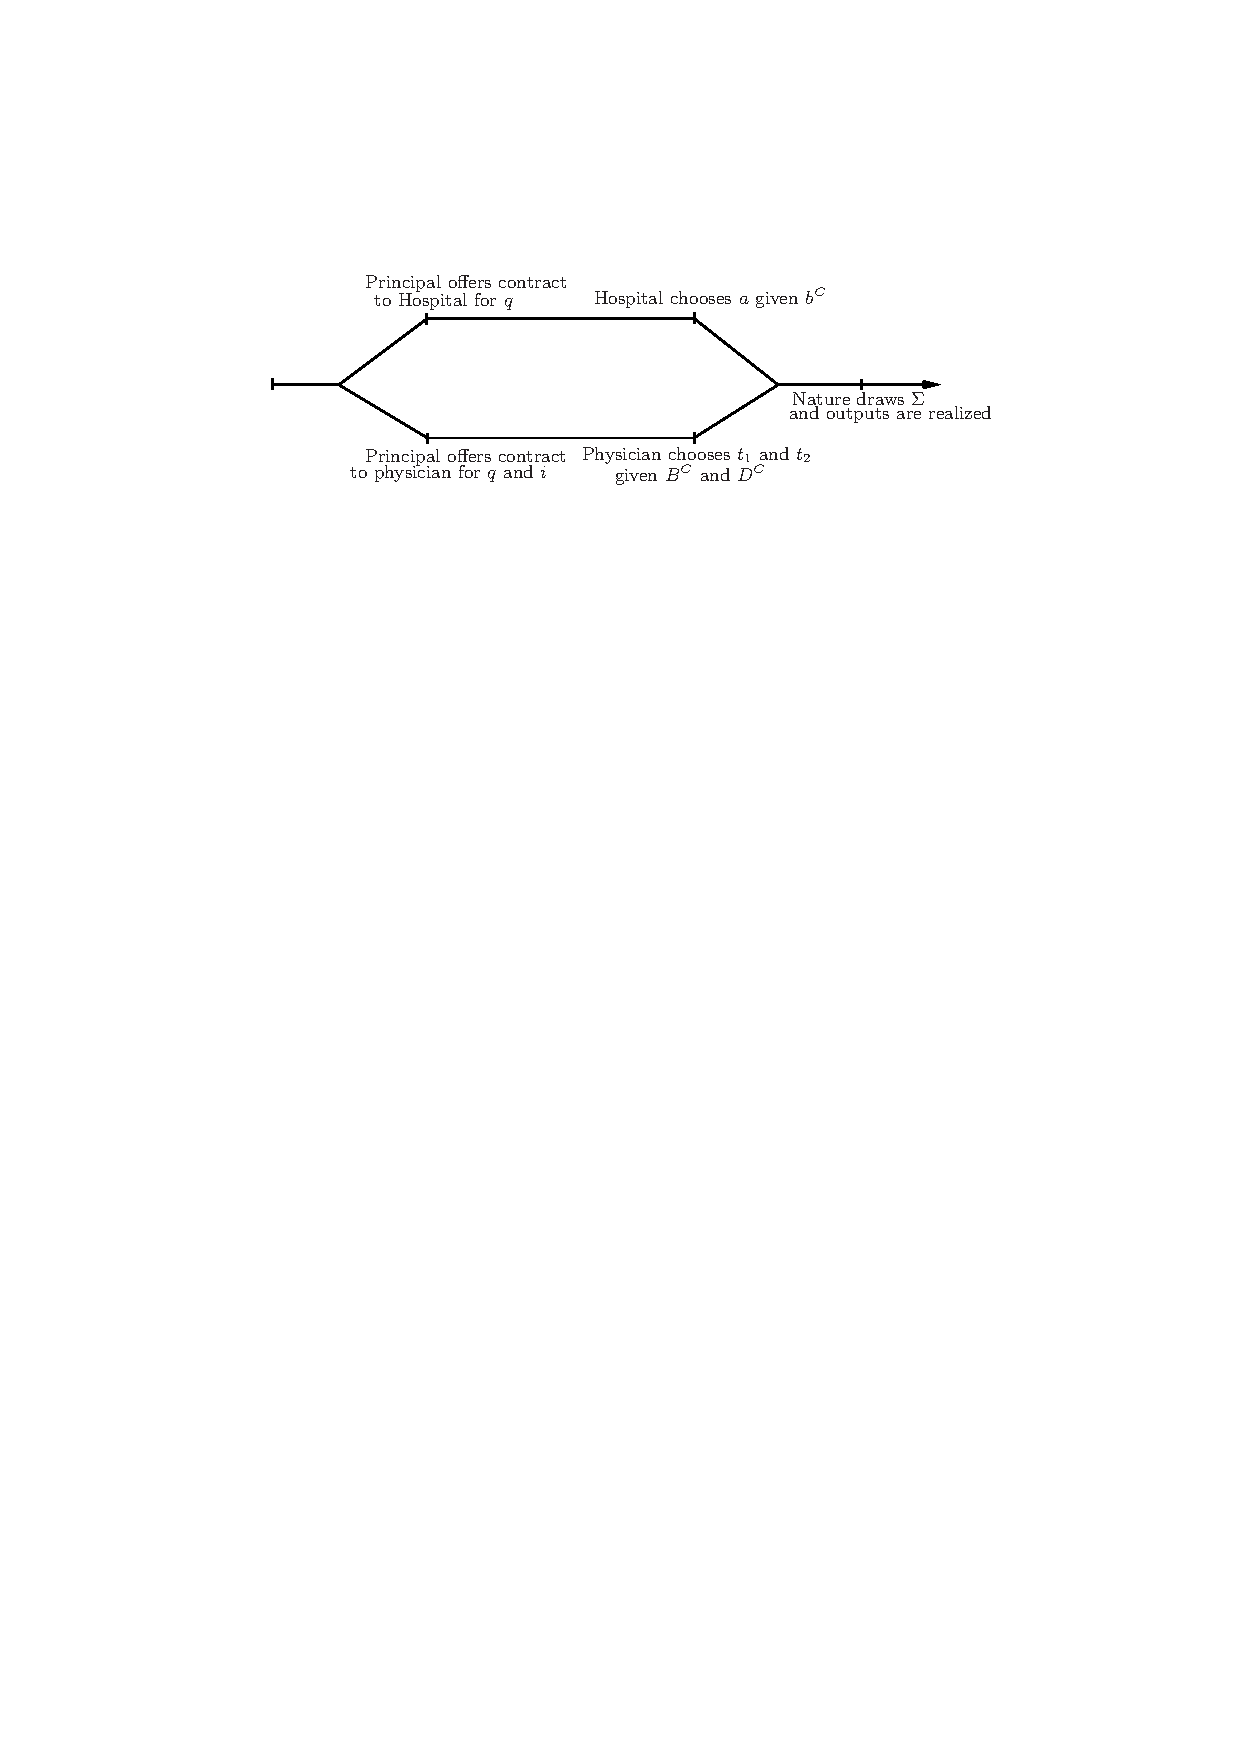
\includegraphics[width=0.62\linewidth,height=0.16\textheight,keepaspectratio]{fig00c2-eps-converted-to.pdf}}
  \caption{Cronograma en una estructura centralizada}\label{fig1}
\end{figure}

Con esta nueva configuraci\'on, el problema de optimizaci\'on del principal pasa a ser:
\begin{eqnarray*}
\nonumber   && \max\limits_{q,i,f,b,F,B,D}\
\mathbb{E}_{\mathbold{\epsilon}}[u_f]=\mathbb{E}_{\mathbold{\epsilon}}\text{\Big{\{}}q+i-\lambda[f+bq+
F+Bq+Di]\text{\Big{\}}}\\
\nonumber &&\text{sujeto a}\\
&&\mathbb{E}_{\mathbold{\epsilon}}[u_h]=\mathbb{E}_{\epsilon_1}[-\e^{-\rho[f+bq-\frac{1}{2}\tau
a^2+z(a)]}]
\geq u_h(\bar{b})\label{ir_h}\\
&&\mathbb{E}_{\mathbold{\epsilon}}[u_m]=\mathbb{E}_{\mathbold{\epsilon}}[-\e^{-\eta[F+Bq+Di-\frac{1}{2}(\psi_1t_1^2+
\psi_2t_2^2)-\psi_{12}t_1t_2+\phi(t_1,t_2)]}] \geq u_m(\bar{w})\label{ir_m}\\
&&a\in argmax_{a}\mathbb{E}_{\epsilon_1}[-\e^{-\rho[f+bq-\frac{1}{2}\tau
a^2+z(a)]}]\label{ic_h}\\
&&t_1,t_2 \in argmax_{t_1,t_2}\mathbb{E}_{\mathbold{\epsilon}}[-\e^{-\eta[F+Bq+Di-\frac{1}{2}(\psi_1t_1^2+ \psi_2t_2^2)-\psi_{12}t_1t_2+\phi(t_1,t_2)]}]\label{ic_m}
\end{eqnarray*}
Las dos primeras restricciones son las de participaci\'on o racionalidad, y la tercera y la cuarta son las restricciones de compatibilidad de incentivos sobre el esfuerzo de los agentes. Utilizando el enfoque de primer orden y la definici\'on de equivalentes ciertos\footnote{En el caso del m\'edico tenemos que $\mathbb{E}_{\mathbold{\epsilon}}[u_m]=-\e^{-\eta\widehat{w}(t_1,t_2)}$, siendo $\widehat{w}(t_1,t_2)=F+B(\bar{a}+t_1)+Dt_2+\phi_1t_1+\phi_2t_2-\frac{1}{2}(\psi_1t_1^2+\psi_2t_2^2)-\psi_{12}t_1t_2-\frac{\eta}{2}(B^2\sigma_1^2+D^2\sigma_2^2+2BD\sigma_{12}^2)$ su renta equivalente cierta para una realizaci\'on dada de $a$. Para el hospital, el equivalente cierto es $ \widehat{b}(a)=f+b(a+\bar{t_1})+z_1a-\frac{1}{2}\tau a^2-\frac{\rho}{2}b^2\sigma_1^2$ dados los valores de $t_1$ y $t_2$.}, obtenemos que:
\begin{eqnarray*}
b^C&=&\tau a-z_1\\
B^C&=&\psi_1t_1+\psi_{12}\bar{t}_2-\phi_1\\
D^C&=&\psi_2t_2 +\psi_{12}\bar{t}_1-\phi_2
\end{eqnarray*}
y resolver los niveles de esfuerzo de \emph{segundo best} da lugar a:
\begin{eqnarray}
a^{C}&=&\frac{b+z_1}{\tau}\label{aso}\\
t_1^{C}&=&\frac{(B+\phi_1)\psi_2-(D+\phi_2)\psi_{12}}{\psi_1\psi_2-\psi_{12}^2}\label{t1so}\\
t_{{2}}^{C}&=&\frac { \left( D+\phi_{{2}} \right) \psi_{{1}}- \left( B+\phi _{{1}} \right)\psi_{{12}}}{\psi_1\psi_2-\psi_{12}^2}\label{t2so}
\end{eqnarray}
El principal fija entonces los componentes fijos de los mecanismos de pago de modo que las restricciones de participaci\'on sean vinculantes (lo que significa que en el \^optimo $ \bar{b}=\widehat{b} $ y $\bar{w}=\widehat{w} $) y los esquemas de compensaci\'on pasan a ser:
\begin{eqnarray*}
 H(q) &=& \bar{b}+\frac{1}{2}\tau a^2-z_1a+\frac{\rho}{2}b^2\sigma_1^2\\
  M(q,i) &=& \bar{w}+\frac{1}{2}(\psi_1t_1^2+\psi_2t_2^2)+\psi_{12}t_1t_2-\phi_1t_1-\phi_2t_2+\frac{\eta}{2}(B^2\sigma_1^2+D^2\sigma_2^2+2DB\sigma_{12}^2)
\end{eqnarray*}
Ahora el problema de optimizaci\'on puede expresarse de la siguiente manera:
\begin{eqnarray*}
\max\limits_{q,i,b,B,D}\ \mathbb{E}_{\mathbold{\epsilon}}[u_f]&=&a+t_1+t_2-\lambda(H(q)+M(q,i))\\
\nonumber \text{sujeto a }&&\\
a&=a^{C}=&\frac{b+z_1}{\tau}\\
t_1&=t_1^{C}=&\frac{(B+\phi_1)\psi_2-(D+\phi_2)\psi_{12}}{\psi_1\psi_2-\psi_{12}^2}\\
t_2&=t_2^{C}=&\frac { \left( D+\phi_{{2}} \right) \psi_{{1}}- \left( B+\phi _{{1}} \right)\psi_{{12}}}{\psi_1\psi_2-\psi_{12}^2}
\end{eqnarray*}

Suponiendo que ambos componentes aleatorios de los outputs se distribuyen independientemente ($\sigma_{12}=0$) y resolviendo el problema de optimizaci\'on del principal obtenemos las expresiones de segundo best para la potencia de los incentivos:
\begin{eqnarray}
b^C&=&\frac {1}{\lambda(1+\rho\sigma_1^2\tau)}\label{bso}\\
B^C&=&\frac{\psi_2-\psi_{12}(1-\lambda D^C)}{\lambda[\psi_2+\eta\sigma_1^2(\psi_1\psi_2-\psi_{12}^2)]}\label{Bso1}\\
D^C&=&\frac{\psi_1-\psi_{12}(1-\lambda B^C)}{\lambda[\psi_1+\eta\sigma_2^2(\psi_1\psi_2-\psi_{12}^2)]}\label{Dso1}
\end{eqnarray}

Resolviendo las ecuaciones \ref{Bso1} y \ref{Dso1} para $B^C$ y $D^C$ obtenemos:
\begin{eqnarray}
B^C&=&\frac{1+\eta\sigma_2^2(\psi_2-\psi_{12})}{\lambda[1+\sigma_1^2\sigma_2^2\eta^2(\psi_1\psi_2-\psi_{12}^2)+\eta(\sigma_1^2\psi_1+\sigma_2^2\psi_2)]}\label{Bso2}\\
D^C&=&\frac{1+\eta\sigma_1^2(\psi_1-\psi_{12})}{\lambda[1+\sigma_1^2\sigma_2^2\eta^2(\psi_1\psi_2-\psi_{12}^2)+\eta(\sigma_1^2\psi_1+\sigma_2^2\psi_2)]}\label{Dso2}
\end{eqnarray}


Podemos destacar una serie de resultados en la solución bajo estructura centralizada:
\begin{itemize}
  \item A diferencia de la solución de primer \emph{best}, el diseño del contrato no depende del grado de altruismo de los agentes. Por tanto, bajo información asimétrica, el esquema óptimo de pagos es el mismo tanto para hospitales o médicos, sean públicos o privados.
  \item Cuando ambas tareas del médico son sustitutivas ($\psi_{12}>0$), la potencia óptima de los incentivos debería estar directamente relacionada y, por tanto, un aumento del pago incentivador sobre la cantidad debería realinearse con un aumento del pago variable sobre la intensidad.
  \item La potencia de los incentivos es independiente entre agentes. Cambiar los incentivos del hospital no tendría efecto sobre los incentivos del médico.
  \item Cuando la intensidad es difícil de medir (alto $\sigma_2$) y los esfuerzos son sustitutivos perfectos, la solución óptima implica ausencia de incentivos para el médico (un salario fijo) y toda la potencia de los incentivos descansa en el parámetro de pago del hospital.
  \item Si no se utilizan incentivos (solo esquemas de pago fijo), el nivel de esfuerzo del hospital será inferior al de la solución de segundo \emph{best}. El esfuerzo del médico será menor o mayor según sus parámetros tecnológicos y de preferencias (véase el \hl{Appendix} para la demostración). En particular, dado que $\psi_1=\psi_2$ y $\sigma_2>\sigma_1$, entonces el esfuerzo en intensidad será mayor y el esfuerzo en cantidad será menor. Los pagos fijos generarán una cantidad de casos tratados por debajo de la óptima y una intensidad de tratamientos por encima de la óptima.
  \item Bajo un esquema de financiación que solo proporcione incentivos óptimos a la eficiencia en cantidad ($b$ dado por la ecuación (\ref{bso}), $B$ por la ecuación (\ref{Bso2}) y $D=0$), tanto el hospital como el médico proporcionan un mayor nivel de esfuerzo en cantidad, pero el médico infraofrece esfuerzo en intensidad.
  \item Si consideramos un tipo mixto de esquema de pago que incluya la potencia óptima de incentivos para el hospital ($b^C$ en la ecuación (\ref{bso})) pero ninguna para el médico ($B=D=0$), entonces, dependiendo otra vez de los valores de los parámetros, deberíamos observar tanto infraprovisión de cantidad como de intensidad.
  \item En una estructura centralizada podemos comparar los niveles multi-output bajo distintos mecanismos de pago incentivador en relación con una línea de base de pago puramente fijo y sin incentivos (por ejemplo, el sistema tradicional retrospectivo o de reembolso de costes).
\end{itemize}

\subsection{Estructura descentralizada}

En una estructura descentralizada, el principal (el financiador) contrata solo con el hospital para un determinado $q$ e $i$, y luego es el hospital quien contrata con el médico. El supuesto de información asimétrica se mantiene en este caso también para la relación entre hospital y médico. Resolviendo por inducción hacia atrás, comenzamos con el problema de maximización del hospital. Esto equivale a encontrar los valores de $B$ y $D$ (componentes incentivadores del pago del médico) y de $a$ (nivel de esfuerzo sobre cantidad proporcionado por el hospital) dados los parámetros fijados por el principal que remuneran los niveles multi-output del hospital ($b$ y $d$). Dados los niveles de esfuerzo de segundo \emph{best}, procedemos resolviendo el problema de optimización del principal. La Figura \ref{fig2} muestra la secuencia temporal en esta estructura organizativa.

\begin{figure}[htbp!]
  \centering
  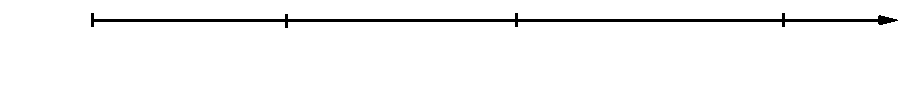
\includegraphics[width=15cm]{fig00d.pdf}
  \caption{Cronograma en una estructura descentralizada}\label{fig2}
\end{figure}

\newpage

El problema del hospital expresado con los correspondientes equivalentes ciertos es, por tanto:
\begin{eqnarray*}
\max\limits_{a,B,D}\ \mathbb{E}_{\mathbold{\epsilon}}[u_h]&=&
f+ \left( b-B \right)  \left( a+t_{{1}} \right) + \left( d-D \right) t_{{2}}+z_{{1}}a-M\\
\nonumber \text{sujeto a }&&\\
t_1=t_1^{D}&=&\frac{(B+\phi_1)\psi_2-(D+\phi_2)\psi_{12}}{\psi_1\psi_2-\psi_{12}^2}\\
t_2=t_2^{D}&=&\frac {\left( D+\phi_{{2}} \right) \psi_{{1}}- \left( B+\phi _{{1}} \right)}{\psi_1\psi_2-\psi_{12}^2}\\
\hat{w}&=&\bar{w}
\end{eqnarray*}

Donde $M=\frac{\tau\,{a}^{2}}{2}+\frac{1}{2}\rho\left((b-B)^2\sigma_1^2+(d-D)^2\sigma_2^2+2(b-B)(d-D)\sigma_{12}^2 \right)+F$ es el coste total del hospital basado en tres componentes: coste de esfuerzo, prima de riesgo y el componente fijo del pago al médico, $F$ (este último se fija de manera que el médico pueda alcanzar su utilidad de reserva).\footnote{$F=\bar{w}-B \left( a+t_{{1}} \right) -\phi_{{1}}t_{{1}}- Dt_{{2}}-\phi_{{2}}t_{{2}}+\frac{1}{2}\,\left(\psi_{{1}}{t_{{1}}}^{2}+\psi_{{2}}{t_{{2}}}^{2}\right)+\psi_{{12}}t_{{1}}t_{{2}}+\frac{\eta}{2}\left( {B}^{2}{\sigma_{{1}}}^{2}+2\,BD{\sigma_{{12}}}^{2}+{D}^{2}{\sigma_{{2}}}^{2} \right)$}

Denotando la suma de los coeficientes de aversión al riesgo por $\theta=(\rho + \eta)$ y $\delta={\psi_1\psi_2-\psi_{12}^2}$, los componentes óptimos de pago variable al médico vienen dados por:
\begin{eqnarray*}
B^D&=&\frac{b(1+\sigma_1^2\rho\psi_1+\sigma_2^2\theta(\rho\delta\sigma_1^2+\psi_2))-d\eta\sigma_2^2\psi_{12}}{1+\psi_1\theta\sigma_1^2+\theta\sigma_2^2\left(\theta\delta\sigma_1^2+\psi_2\right)}\\
D^D&=&\frac{d(1+\sigma_2^2\rho\psi_2+\sigma_1^2\theta(\rho\delta\sigma_2^2+\psi_1))-b\eta\sigma_2^2\psi_{12}}{1+\psi_2\theta\sigma_2^2+\theta\sigma_1^2\left( \theta\,\delta\sigma_2^2+\psi_1\right)}
\end{eqnarray*}
Resolviendo para $t_1$ y $t_2$ dados los valores de $B$ y $D$, obtenemos los esfuerzos de segundo \emph{best} del médico, $t_1(b,d)$ y $t_2(b,d)$, que el hospital incentivará en función de sus propios parámetros de pago.

El problema de optimización del principal viene ahora dado por:
\begin{eqnarray*}
  \max\limits_{q,i,b,d}\ \mathbb{E}_{\mathbold{\epsilon}}[u_f]&=&a+t_1+t_2-\lambda\left (f+b(a+t_1)+dt_2\right ) \\
  a^D&=&\frac{b+z_1}{\tau}\\
  t_1^D &=& t_1(b,d) \\
  t_2^D &=& t_2(b,d)\\
  \hat{b}&=&\bar{b}
\end{eqnarray*}
donde $f=\bar{b}-(b-B)(a+t_1)-(d-D)t_2-z_1a-M$ es el componente fijo del esquema del hospital que hace vinculante su restricción de participación. La solución de este programa es un objeto complicado que depende de los parámetros fundamentales. Para el caso especial de tareas independientes en la función de costes del médico ($\psi_{12}=0$), los parámetros óptimos de pago en los componentes variables son fijados por hospital y principal de acuerdo con las siguientes expresiones:
\begin{eqnarray*}
  B^D &=& {\frac { \left( {\sigma_{{1}}}^{2}\theta\,{\psi_{{1}}}^{2}+ \left(\rho\,\tau\,{\sigma_{{1}}}^{2}+1 \right) \psi_{{1}}+\tau \right)
 \left( \rho\,\psi_{{1}}{\sigma_{{1}}}^{2}+1 \right) }{ \left( {\sigma
_{{1}}}^{2} \left( \eta\,\rho\,\tau\,{\sigma_{{1}}}^{2}+\eta+\rho
 \right) {\psi_{{1}}}^{2}+ \left( \rho\,\tau\,{\sigma_{{1}}}^{2}+1
 \right) \psi_{{1}}+\tau \right) \lambda\, \left( {\sigma_{{1}}}^{2}
\theta\,\psi_{{1}}+1 \right) }} \\
  D ^D&=& {\frac { \left( \rho\,\psi_{{2}}{\sigma_{{2}}}^{2}+1 \right) ^{2}}{
\lambda\, \left( {\sigma_{{2}}}^{2}\theta\,\psi_{{2}}+1 \right)
 \left( \eta\,\rho\,{\psi_{{2}}}^{2}{\sigma_{{2}}}^{4}+\rho\,\psi_{{2}
}{\sigma_{{2}}}^{2}+1 \right) }}\\
  b^D &=& {\frac {{\sigma_{{1}}}^{2}\theta\,{\psi_{{1}}}^{2}+ \left( \rho\,\tau
\,{\sigma_{{1}}}^{2}+1 \right) \psi_{{1}}+\tau}{ \left( {\sigma_{{1}}}
^{2} \left( \eta\,\rho\,\tau\,{\sigma_{{1}}}^{2}+\eta+\rho \right) {
\psi_{{1}}}^{2}+ \left( \rho\,\tau\,{\sigma_{{1}}}^{2}+1 \right) \psi_
{{1}}+\tau \right) \lambda}}\\
  d^D &=& {\frac {\rho\,\psi_{{2}}{\sigma_{{2}}}^{2}+1}{ \left( 1+ \left( \eta
\,{\psi_{{2}}}^{2}{\sigma_{{2}}}^{4}+\psi_{{2}}{\sigma_{{2}}}^{2}
 \right) \rho \right) \lambda}}
\end{eqnarray*}

Como puede verse, los parámetros altruistas no entran en el componente de pago como ocurría en la estructura centralizada. Los niveles óptimos de esfuerzo tanto para el hospital como para el médico son\footnote{Para compactar la solución supondremos que no existe interés altruista ni en el hospital ni en el médico, es decir, $z_1=\phi_1=\phi_2=0$.}:
\begin{eqnarray*}
a^D&=&{\frac {{\sigma_{{1}}}^{2}\theta\,{\psi_{{1}}}^{2}+ \left( \rho\,\tau
\,{\sigma_{{1}}}^{2}+1 \right) \psi_{{1}}+\tau}{\tau\,\lambda\,
 \left( {\sigma_{{1}}}^{2} \left( \eta\,\rho\,\tau\,{\sigma_{{1}}}^{2}
+\eta+\rho \right) {\psi_{{1}}}^{2}+ \left( \rho\,\tau\,{\sigma_{{1}}}
^{2}+1 \right) \psi_{{1}}+\tau \right) }}\\
t_1^D&=&{\frac { \left( \rho\,\psi_{{1}}{\sigma_{{1}}}^{2}+1 \right)  \left( {
\sigma_{{1}}}^{2}\theta\,{\psi_{{1}}}^{2}+ \left( \rho\,\tau\,{\sigma_
{{1}}}^{2}+1 \right) \psi_{{1}}+\tau \right) }{\lambda\,\psi_{{1}}
 \left( \theta\,\psi_{{1}}{\sigma_{{1}}}^{2}+1 \right)  \left( {\sigma
_{{1}}}^{2} \left(  \left( \eta\,\tau\,{\sigma_{{1}}}^{2}+1 \right)
\rho+\eta \right) {\psi_{{1}}}^{2}+ \left( \rho\,\tau\,{\sigma_{{1}}}^
{2}+1 \right) \psi_{{1}}+\tau \right) }}\\
t_2^D&=& {\frac { \left( \rho\,\psi_{{2}}{\sigma_{{2}}}^{2}+1 \right) ^{2}}{
\lambda\,\psi_{{2}} \left( 1+ \left( \eta\,{\psi_{{2}}}^{2}{\sigma_{{2
}}}^{4}+\psi_{{2}}{\sigma_{{2}}}^{2} \right) \rho \right)  \left( \eta
\,\psi_{{2}}{\sigma_{{2}}}^{2}+\rho\,\psi_{{2}}{\sigma_{{2}}}^{2}+1
 \right) }}
\end{eqnarray*}
Si comparamos estos resultados con los de la estructura centralizada:
\begin{eqnarray*}
  a^C &=& {\frac {1}{\lambda\, \left( \rho\,\tau\,{\sigma_{{1}}}^{2}+1 \right)
\tau}}\\
  t_1^C &=& {\frac {1}{ \left( \eta\,\psi_{{1}}{\sigma_{{1}}}^{2}+1 \right)
\lambda\,\psi_{{1}}}} \\
  t_2^C &=& {\frac {1}{\psi_{{2}}\lambda\, \left( \eta\,\psi_{{2}}{\sigma_{{2}}}^{2}+1 \right) }}
\end{eqnarray*}
podemos observar que la estructura centralizada produce soluciones mucho más simples para los pagos incentivadores. Puede demostrarse (véase el \hl{Appendix}) que el nivel de esfuerzo del hospital es mayor en la estructura descentralizada ($a^D>a^C$), mientras que el nivel de esfuerzo en intensidad del médico es menor ($t_2^D<t_2^C$). Para que el esfuerzo del médico en cantidad sea mayor bajo la estructura centralizada, debe cumplirse que $\eta\tau\sigma_1^2>1+\sigma_1^2\theta\psi_1$. Esto significa que, dados $\sigma_1$ y los coeficientes de aversión al riesgo de los agentes ($\eta$ y $\rho$), para un coste suficientemente mayor de producir $q$ por parte del hospital en relación con ese mismo coste para el médico, la cantidad proporcionada por el médico en una estructura centralizada será mayor que en una descentralizada\footnote{Sin embargo, es inmediato ver que cuando $\psi_1>\tau$ entonces $t_1^D>t_1^C$.}. En otras palabras, cuando las tareas son independientes en la función de costes del médico y su coste marginal de atender a más pacientes es suficientemente menor que el del hospital, una estructura centralizada con esquemas compatibles con incentivos mostrará mayor intensidad en los tratamientos y un mayor volumen de pacientes atendidos. No obstante lo anterior, nos interesa una comparación más rica entre el desempeño de los agentes en distintos entornos organizativos. Utilizando valores dados de los parámetros fundamentales del modelo, procederemos ahora a analizar, mediante ilustraciones gráficas, la potencia diferencial de los incentivos y los resultados de esfuerzo entre las dos formas de estructurar las relaciones contractuales.

\section{Comparación de estructuras organizativas}
La forma compleja de la solución (especialmente en el caso descentralizado) no permite una comparación limpia de las interrelaciones entre los esquemas óptimos de incentivos y los niveles óptimos de esfuerzo en ambos marcos jerárquicos. Para derivar algunos resultados generales sobre la naturaleza de la interdependencia entre tareas o sobre el efecto de las variaciones del ruido en la medida de cantidad o intensidad, trabajaremos con simulaciones gráficas para distintos escenarios\footnote{Todos los gráficos se construyen para valores unitarios en el resto de parámetros, salvo cuando se indique otra cosa.}. Consideremos primero el efecto de un cambio en $\psi_{12}$ tanto sobre los parámetros de incentivos como sobre la diferencia entre niveles de esfuerzo. Luego consideraremos (principalmente para esfuerzos sustitutivos) el cambio en $\sigma_1$ y $\sigma_2$ (la precisión de las señales de resultados).

\subsection{Cambio en la interacción entre tareas}
La Figura \ref{fig3} representa los pagos incentivadores óptimos para una rejilla de valores de $\psi_{12}$ que va desde complementariedad perfecta hasta sustitución perfecta.

\begin{figure}[htbp!]
  \centering
  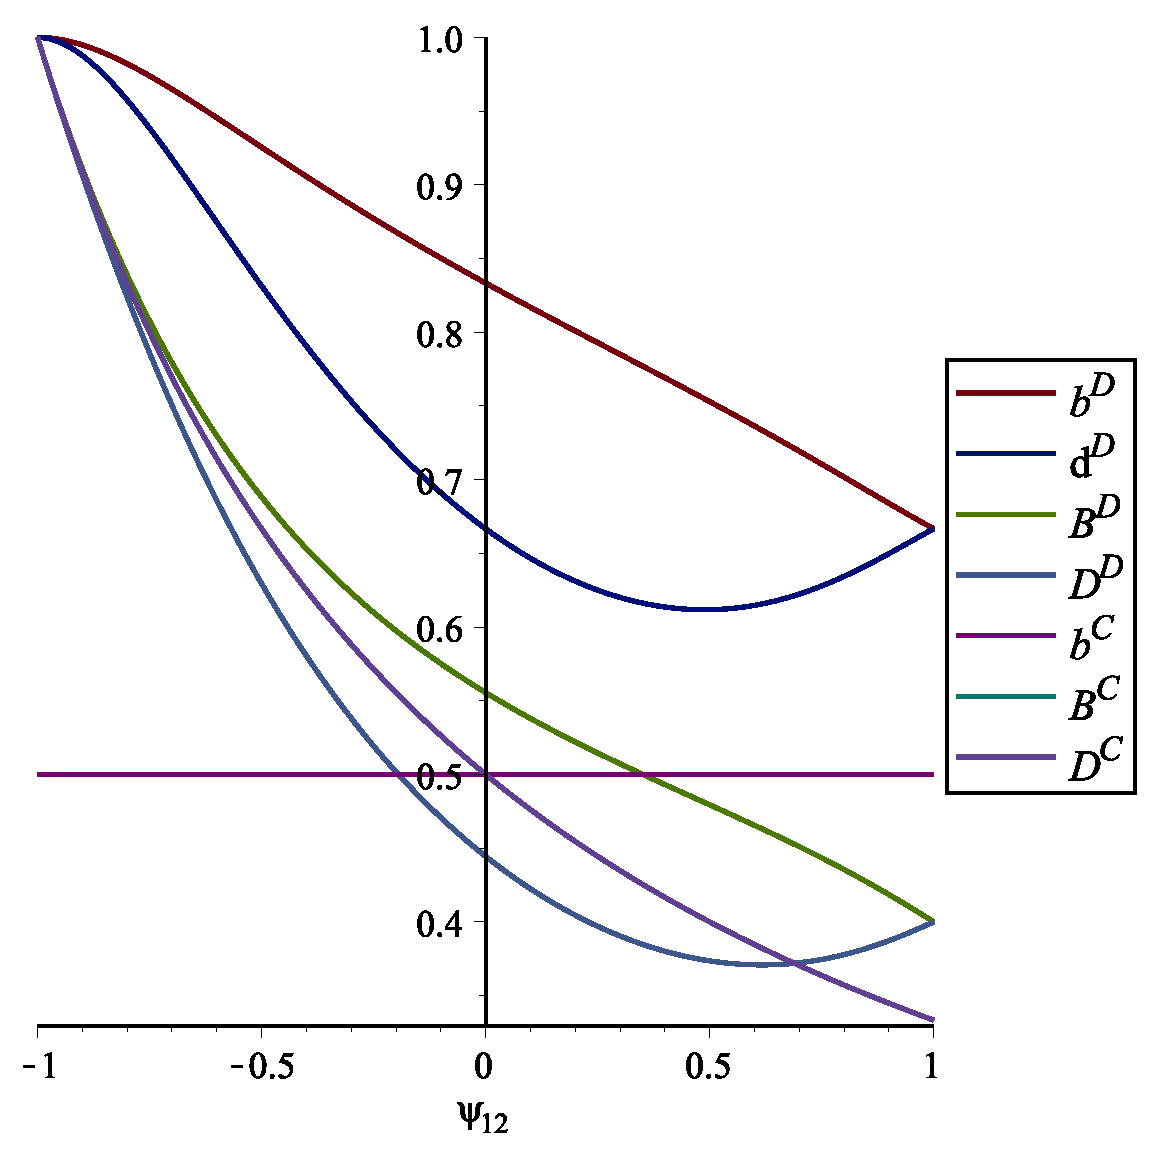
\includegraphics[width=8cm]{gr1-eps-converted-to.pdf}\\
  \caption{Incentivos óptimos con estructuras descentralizada (D) y centralizada (C)}\label{fig3}
\end{figure}
Excepto el pago incentivador constante al hospital cuando el principal solo contrata cantidad con él, todos los pagos variables cambian con la interacción entre las tareas del médico. Cuando los esfuerzos son \emph{complementarios perfectos}, los mecanismos de incentivos alcanzan su máximo (y pasan a ser iguales entre sí) en ambas estructuras. El pago óptimo a la cantidad del hospital en la estructura descentralizada y el correspondiente al esfuerzo del médico sobre la cantidad en ambos marcos disminuyen continuamente a medida que $\psi_{12}$ aumenta. Sin embargo, los pagos por intensidad (tanto para el hospital como para el médico) empiezan a aumentar en cuanto el grado de sustitución alcanza un determinado umbral. Cuando el principal solo contrata con el hospital, la potencia de los incentivos (tanto para hospital como para médico) es mayor en la dimensión de cantidad que en la de intensidad (excepto en los casos extremos de complementariedad perfecta o sustitución perfecta). Aún más interesante es que, aunque en la estructura centralizada todos los pagos variables al médico tienden a cero cuando las tareas tienden a la sustitución perfecta, esto no ocurre en la estructura descentralizada. Como consecuencia, cuando los esfuerzos se vuelven \emph{sustitutivos perfectos}, es óptimo para el financiador (el proveedor público o la aseguradora) no incluir incentivos en el contrato del médico si la configuración es centralizada. Por el contrario, cuando trata exclusivamente con el hospital, el principal incluirá esquemas de incentivos de alta potencia que, posteriormente, \emph{cascadearán} hacia el segundo nivel de arreglos entre hospital y médico. Este resultado podría ayudarnos a ver por qué podría ser óptimo introducir pagos por desempeño para los médicos cuando los hospitales ven ampliado su grado de autonomía. Por el contrario, deberían preferirse salarios fijos o incentivos de baja potencia cuando el principal contrata separadamente con los gestores hospitalarios y con los médicos. \emph{Si las tareas son sustitutivas perfectas, de alguna manera, la adecuación del uso de incentivos bajo riesgo moral parece depender del diseño organizativo vigente.}

Cuando esta distinta potencia de los incentivos se traduce en niveles de esfuerzo, podemos apreciar mejor el efecto diferencial de los dos arreglos organizativos. La Figura \ref{fig4} muestra las diferencias en los niveles óptimos de esfuerzo en la estructura descentralizada respecto de la centralizada. Como se observa, el nivel de cantidad del hospital es siempre mayor en un escenario descentralizado, mientras que el esfuerzo del médico sobre cantidad solo es ligeramente superior en la estructura centralizada para valores muy bajos (y negativos) de $\psi_{12}$. Cuando la complementariedad entre tareas es total, el esfuerzo del médico tanto en cantidad como en intensidad es el mismo en ambos entornos. A medida que los esfuerzos del médico se vuelven cada vez más sustitutivos, su desempeño en cantidad aumenta en el escenario descentralizado en comparación con el centralizado, y lo contrario sucede en la dimensión de intensidad.

\begin{figure}[htbp!]
  \centering
  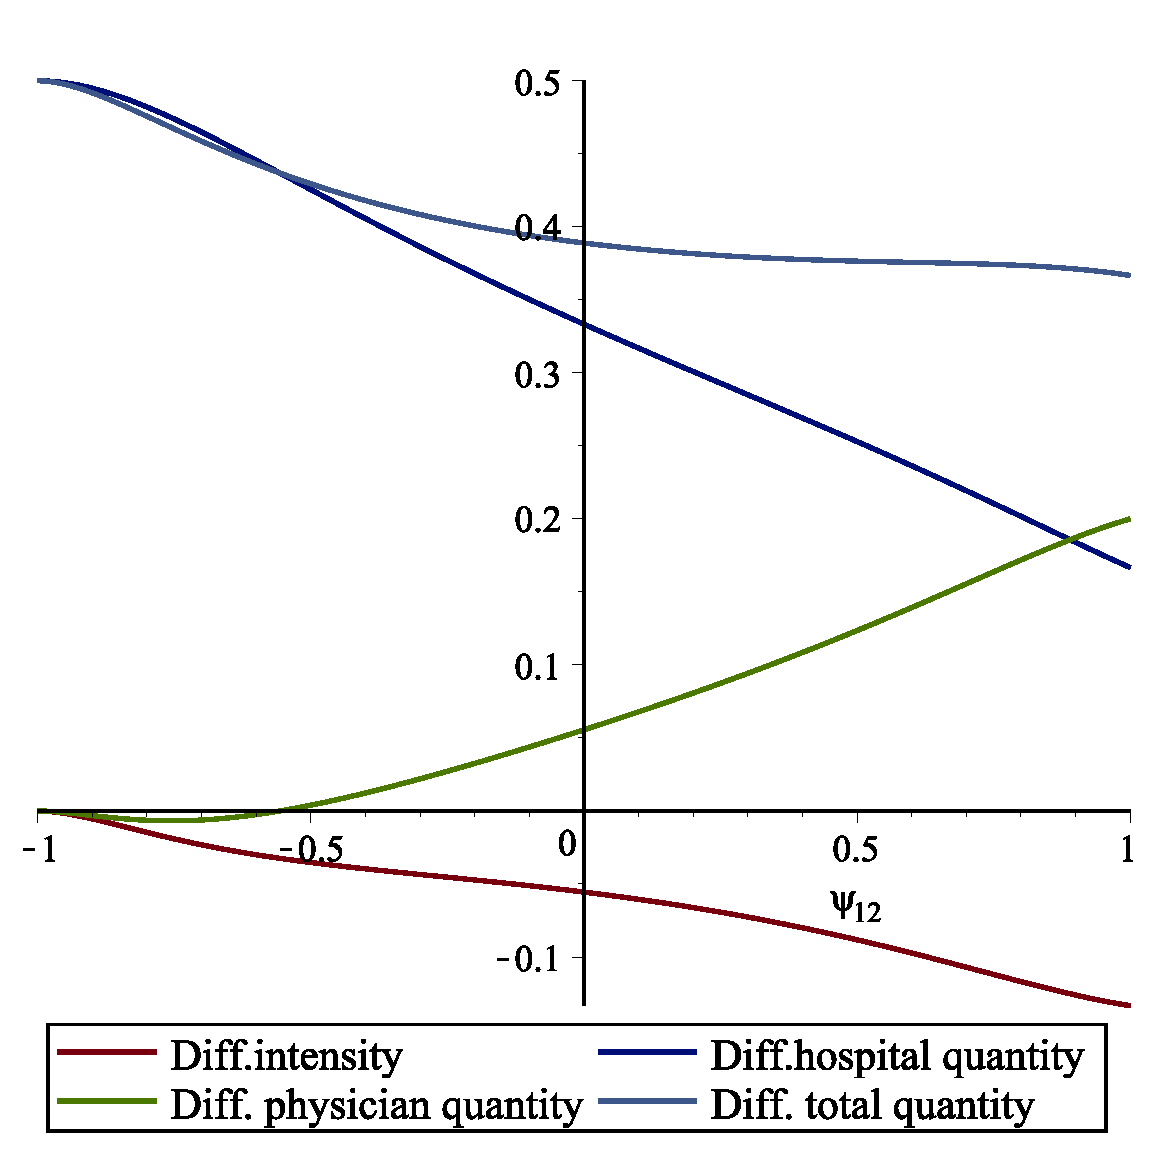
\includegraphics[width=8cm]{gr2-eps-converted-to.pdf}\\
  \caption{Diferencial de esfuerzos (descentralizada frente a centralizada)}\label{fig4}
\end{figure}

El nivel total de esfuerzo en cantidad es mayor cuando el principal solo contrata con el hospital. A medida que las tareas se vuelven cada vez más sustitutivas, la estructura descentralizada desplaza pesos en favor de contratar cantidad del médico en lugar del hospital, y la estructura centralizada hace lo contrario. Esto debería ser resultado de una estructura centralizada que reduce la potencia de los incentivos con $\psi_{12}$, como se ha mostrado arriba.

Si el nivel de cantidad está completamente determinado por el nivel de esfuerzo de los agentes, es decir, $\sigma_1=0$, la intensidad sigue siendo menor en el caso descentralizado, pero ahora la diferencia en los niveles de esfuerzo sobre cantidad, tanto del hospital como del médico, se compensa completamente, de modo que la cantidad total es la misma en las dos estructuras y alcanza valores de primer \emph{best}. Por otro lado, cuando es la intensidad del tratamiento la que se mide sin ninguna señal ruidosa ($\sigma_2=0$), los insumos de cantidad son mayores en la estructura descentralizada tanto para hospital como para médico e independientes de la interacción entre tareas, y ahora la intensidad es la misma que en el escenario de información simétrica en ambas estructuras. Las Figuras \ref{fig5} y \ref{fig6} presentan respectivamente estos dos casos especiales.

\begin{figure}[htbp!]
  \centering
  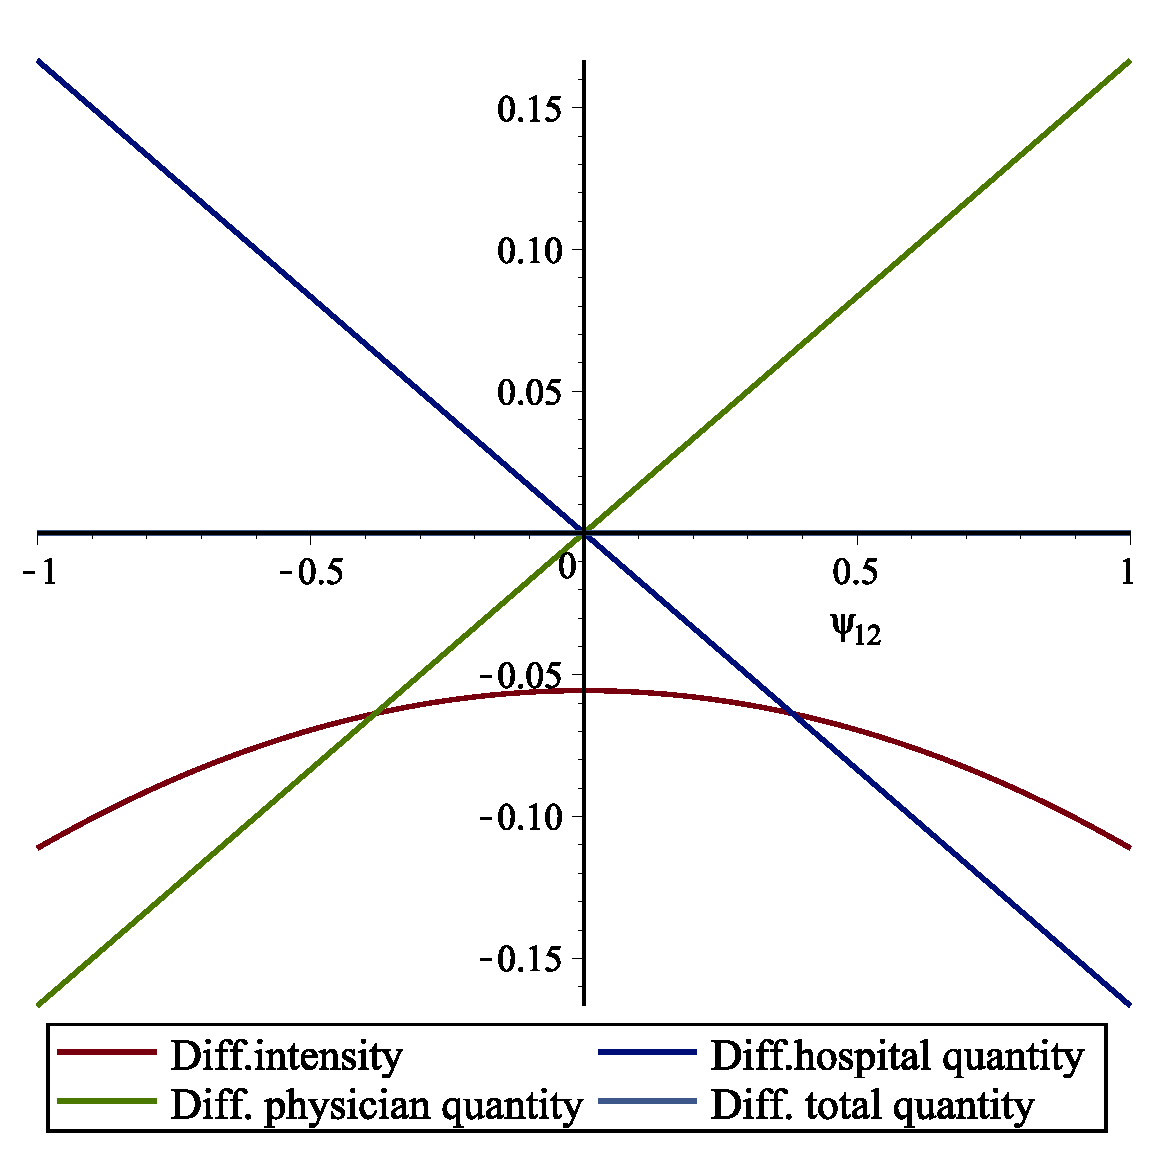
\includegraphics[width=8cm]{gr3-eps-converted-to.pdf}\\
  \caption{Diferencial de esfuerzos dado $\sigma_1=0$}\label{fig5}
\end{figure}
\begin{figure}[htbp!]
  \centering
  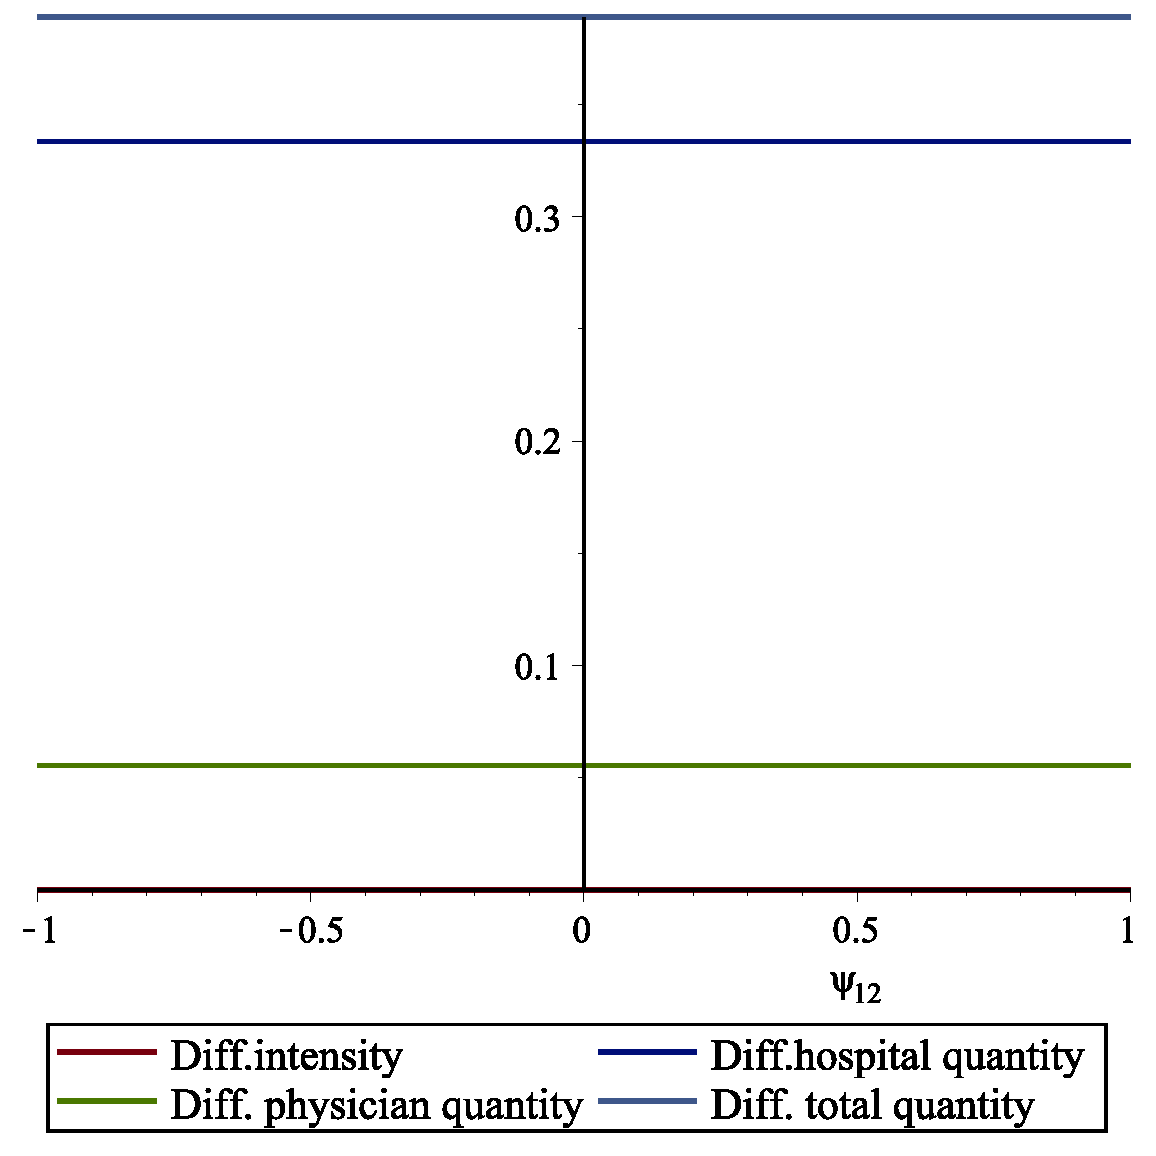
\includegraphics[width=8cm]{gr4-eps-converted-to.pdf}\\
  \caption{Diferencial de esfuerzos dado $\sigma_2=0$.}\label{fig6}
\end{figure}

\subsection{Medición imprecisa de los resultados}

Consideremos ahora la variación en los esquemas de incentivos y en los niveles de esfuerzo cuando, para un valor dado de $\psi_{12}$, la medición de los resultados se vuelve cada vez más imprecisa. La Figura \ref{fig7} muestra cómo cambian los pagos incentivadores variables a medida que la cantidad se vuelve más ruidosa y las tareas del médico son sustitutivas imperfectas ($\psi_{12}=0.5$). Todos los parámetros de incentivos disminuyen a medida que $\sigma_1$ aumenta, pero mientras los pagos variables por cantidad tienden a cero, los pagos por intensidad se estabilizan asintóticamente en un valor positivo independientemente de la estructura organizativa. En suma, a medida que la medición de la cantidad se vuelve cada vez más imprecisa (transfiriendo por tanto más riesgo a los agentes en esa dimensión del output), la potencia de los incentivos, como cabía esperar, disminuye. Los incentivos también disminuyen en la dimensión de intensidad, pero luego tienden asintóticamente a permanecer positivos y constantes.
\begin{figure}[htbp!]
  \centering
  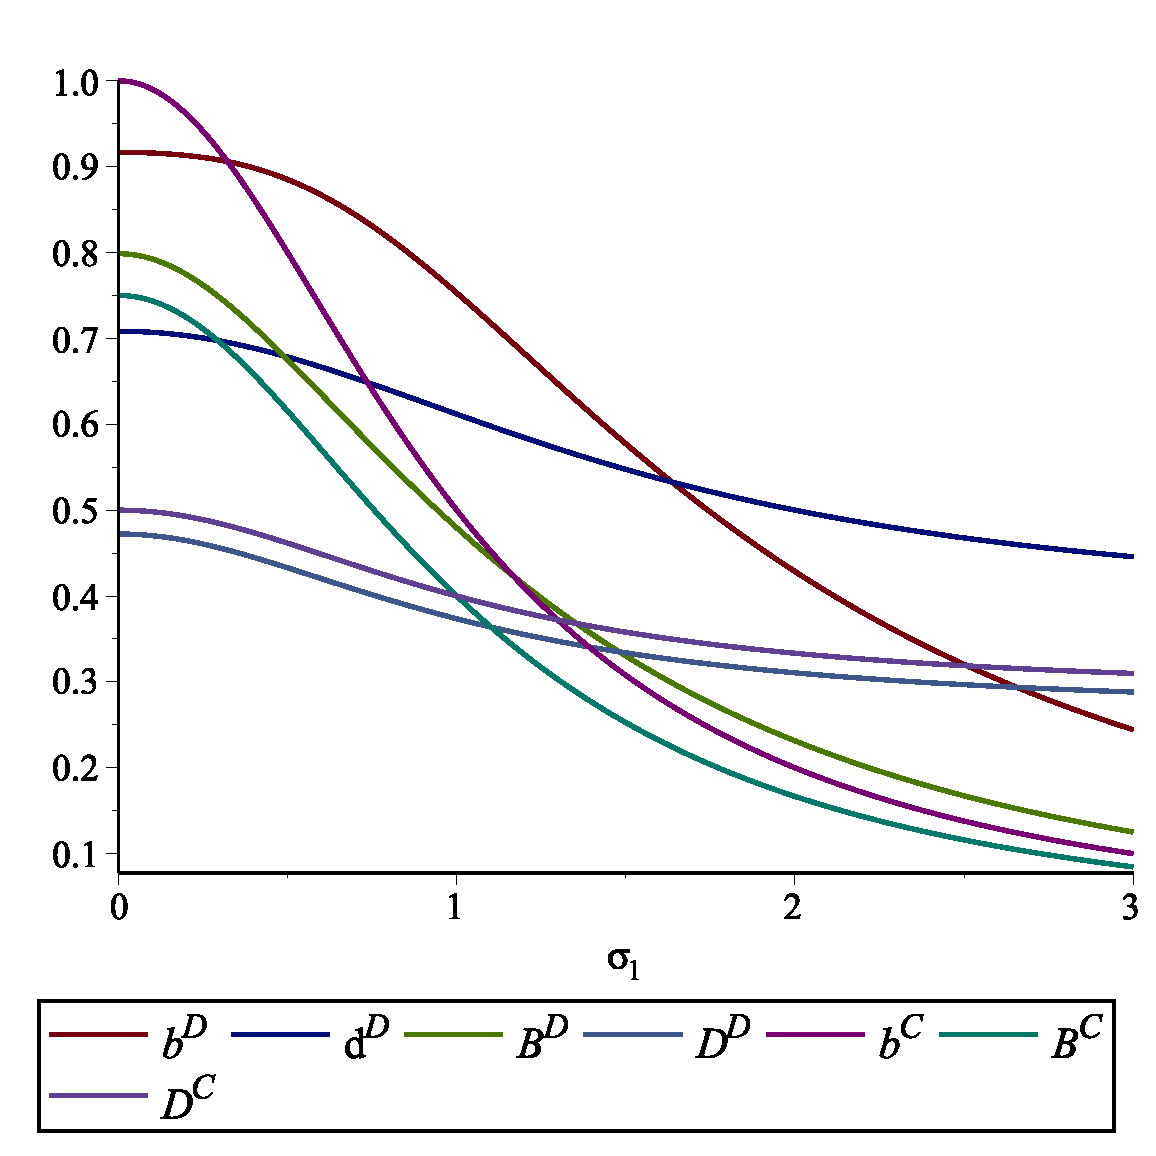
\includegraphics[width=8cm]{gr5-eps-converted-to.pdf}\\
  \caption{Incentivos óptimos cuando aumenta $\sigma_1$.}\label{fig7}
\end{figure}

\begin{figure}[h!]
  \centering
  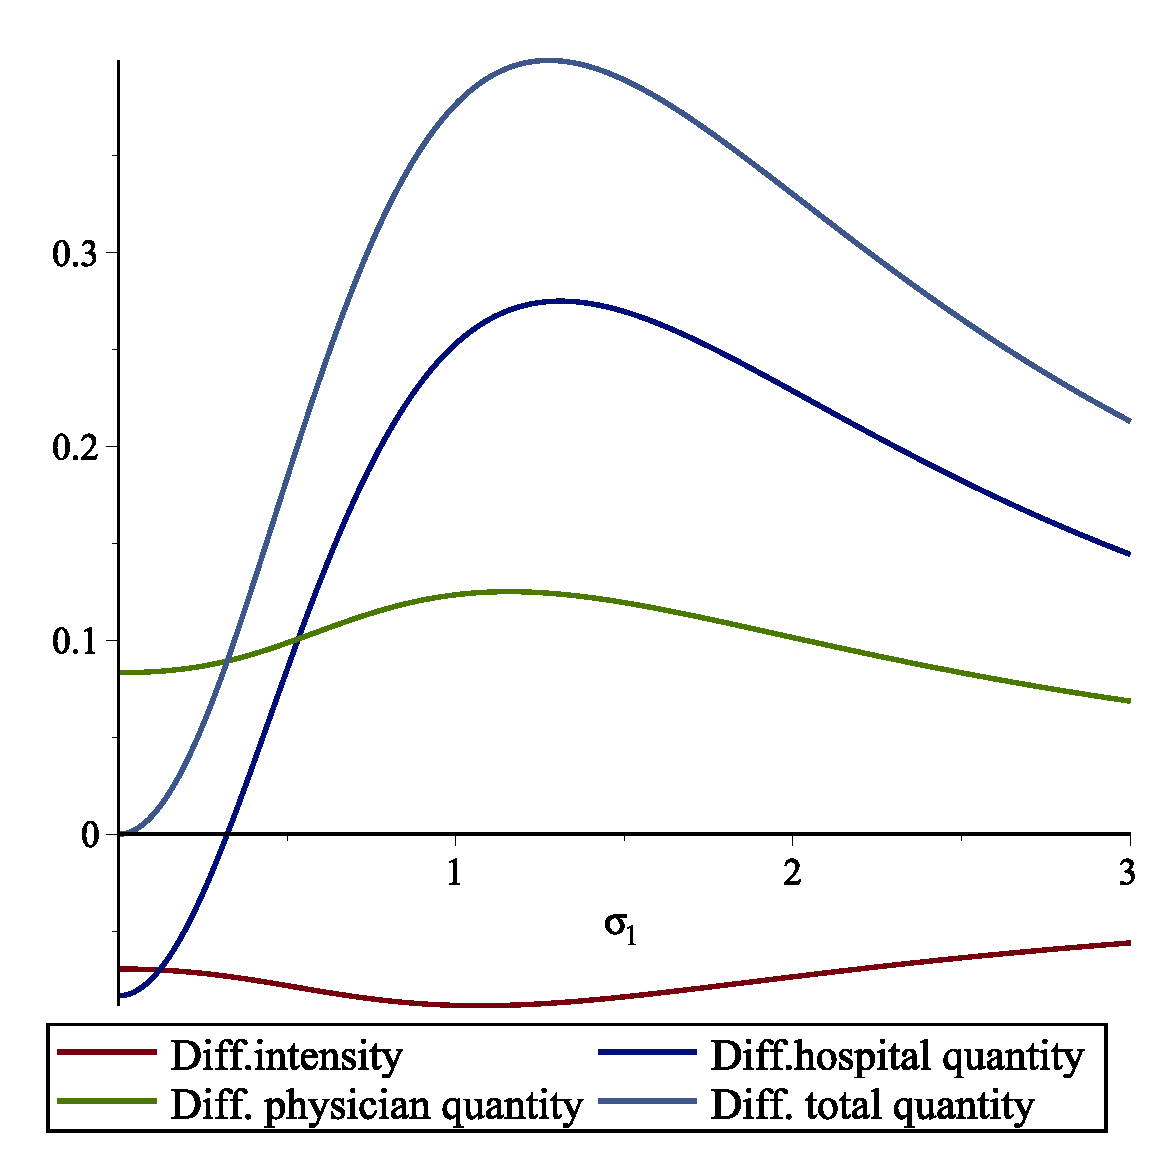
\includegraphics[width=8cm]{gr6-eps-converted-to.pdf}\\
  \caption{Diferencial de esfuerzos cuando aumenta $\sigma_1$.}\label{fig8}
\end{figure}

Dados estos esquemas de incentivos, las diferencias de esfuerzo se representan en la Figura \ref{fig8}. La intensidad sigue siendo mayor bajo una estructura centralizada, pero la cantidad total es mayor bajo una descentralizada. En el límite, los esfuerzos del hospital sobre cantidad tienden a converger en los dos entornos, pero el esfuerzo del médico sobre cantidad permanece más alto en una estructura descentralizada por grande que sea el ruido en la medición de la cantidad. Este mayor esfuerzo del médico sobre cantidad en el caso descentralizado es la única fuerza que impulsa un mayor nivel de cantidad en esa configuración\footnote{Para el caso de complementos imperfectos, sin embargo, tanto el esfuerzo en cantidad como en intensidad pasan, en el límite, a ser mayores en la estructura centralizada a medida que crece el ruido en la medición de la cantidad.}.

Podemos comprobar ahora el efecto sobre incentivos y desempeño cuando, dados los valores del resto de parámetros, el ruido en la medición de la intensidad ($\sigma_2$) aumenta.
La Figura \ref{fig9} muestra cómo todos los incentivos sobre intensidad disminuyen y tienden a cero (más rápidamente para el médico que para el hospital) cuando $\psi_{12}=0.5$. Los incentivos sobre cantidad tienden a disminuir a medida que aumenta el ruido en intensidad (excepto el parámetro del hospital en el caso centralizado, que es independiente de $\sigma_2$), pero para niveles altos de imprecisión en la señal de intensidad todos ellos tienden a estabilizarse y a seguir siendo positivos\footnote{Lo contrario ocurre cuando las tareas son complementarias imperfectas y $\psi_{12}=-0.5$: los incentivos sobre cantidad tienden a cero con $\sigma_2$ y los incentivos sobre intensidad permanecen positivos.}. Puede comprobarse, sin embargo, que la suma de la potencia de los incentivos de ambos agentes es mayor en la estructura descentralizada que en la centralizada\footnote{Interesantemente, cuando las tareas se acercan a la sustitución perfecta, la potencia de los incentivos en el caso descentralizado tiende a cero a medida que crece la imprecisión en los valores de intensidad.}.

\begin{figure}[htbp!]
  \centering
  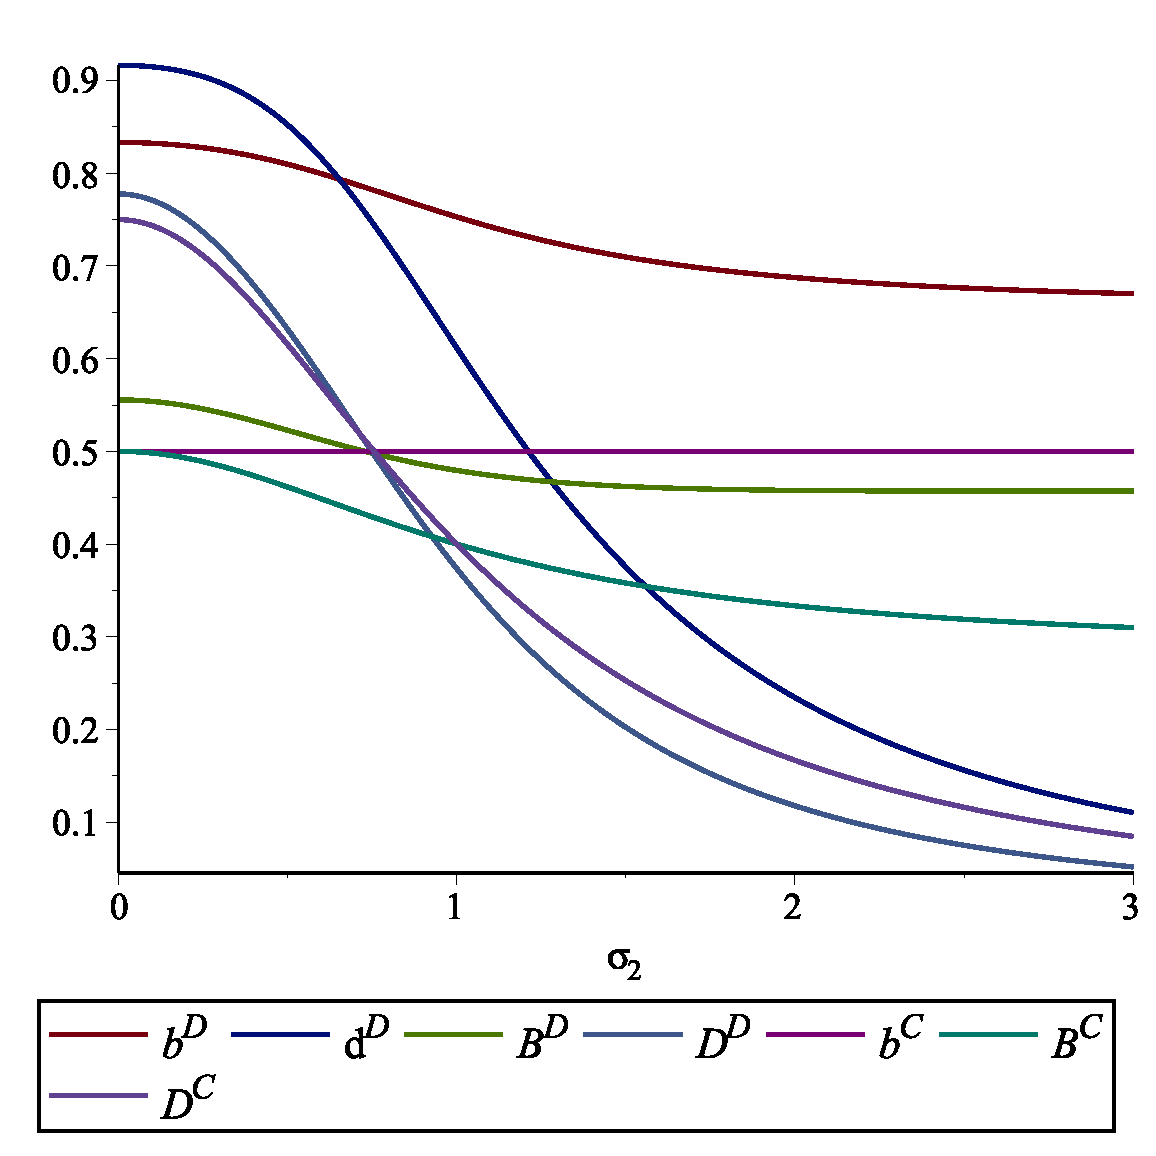
\includegraphics[width=8cm]{gr7-eps-converted-to.pdf}\\
  \caption{Incentivos óptimos cuando aumenta $\sigma_2$.}\label{fig9}
\end{figure}

La interacción de estos esquemas de incentivos con el resto de los parámetros del modelo da lugar a un perfil de diferencias en el desempeño en esfuerzo entre organizaciones que puede analizarse visualmente en la Figura \ref{fig10}.

Para un nivel intermedio de sustitución entre tareas ($\psi_{12}=0.5$), cuando la intensidad se mide sin ruido, los niveles de $t_2$ del médico son iguales y tanto el esfuerzo del médico como el del hospital sobre cantidad son mayores en el caso descentralizado. Pero a medida que $\sigma_2$ tiende a hacerse mayor, la intensidad se reduce en el caso descentralizado respecto de la estructura centralizada. El esfuerzo del hospital sobre cantidad disminuye y el del médico también disminuye, pero ambos siguen siendo mayores cuando el principal solo contrata con el hospital.
\begin{figure}[htbp!]
  \centering
  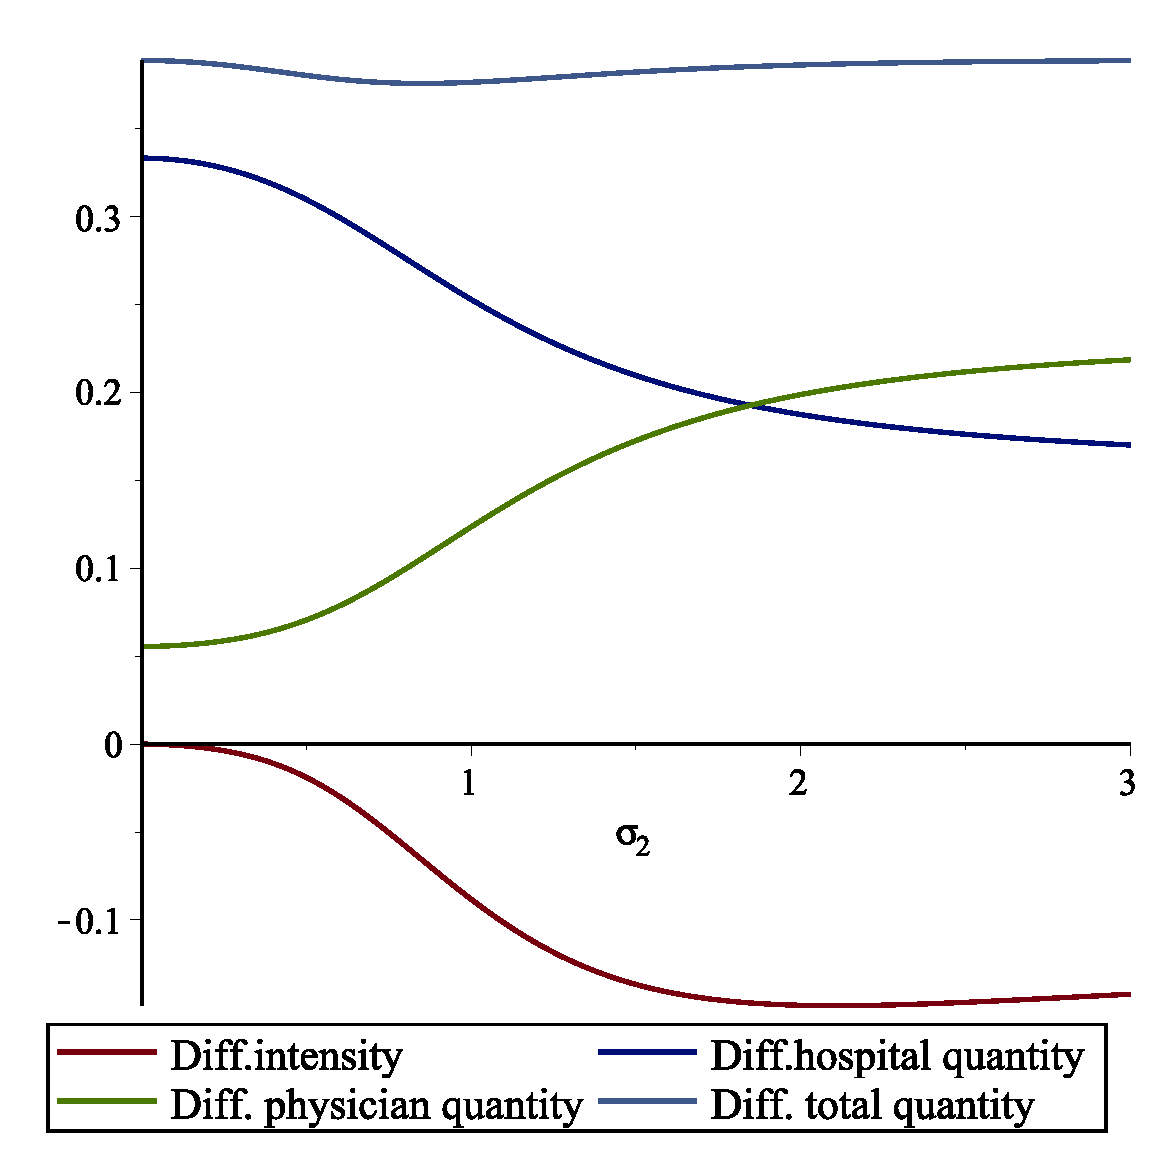
\includegraphics[width=8cm]{gr8-eps-converted-to.pdf}\\
  \caption{Diferencial de esfuerzos cuando aumenta $\sigma_2$ y las tareas son sustitutivas imperfectas ($\psi_{12}=0.5$).}\label{fig10}
\end{figure}

\begin{figure}[htbp!]
  \centering
  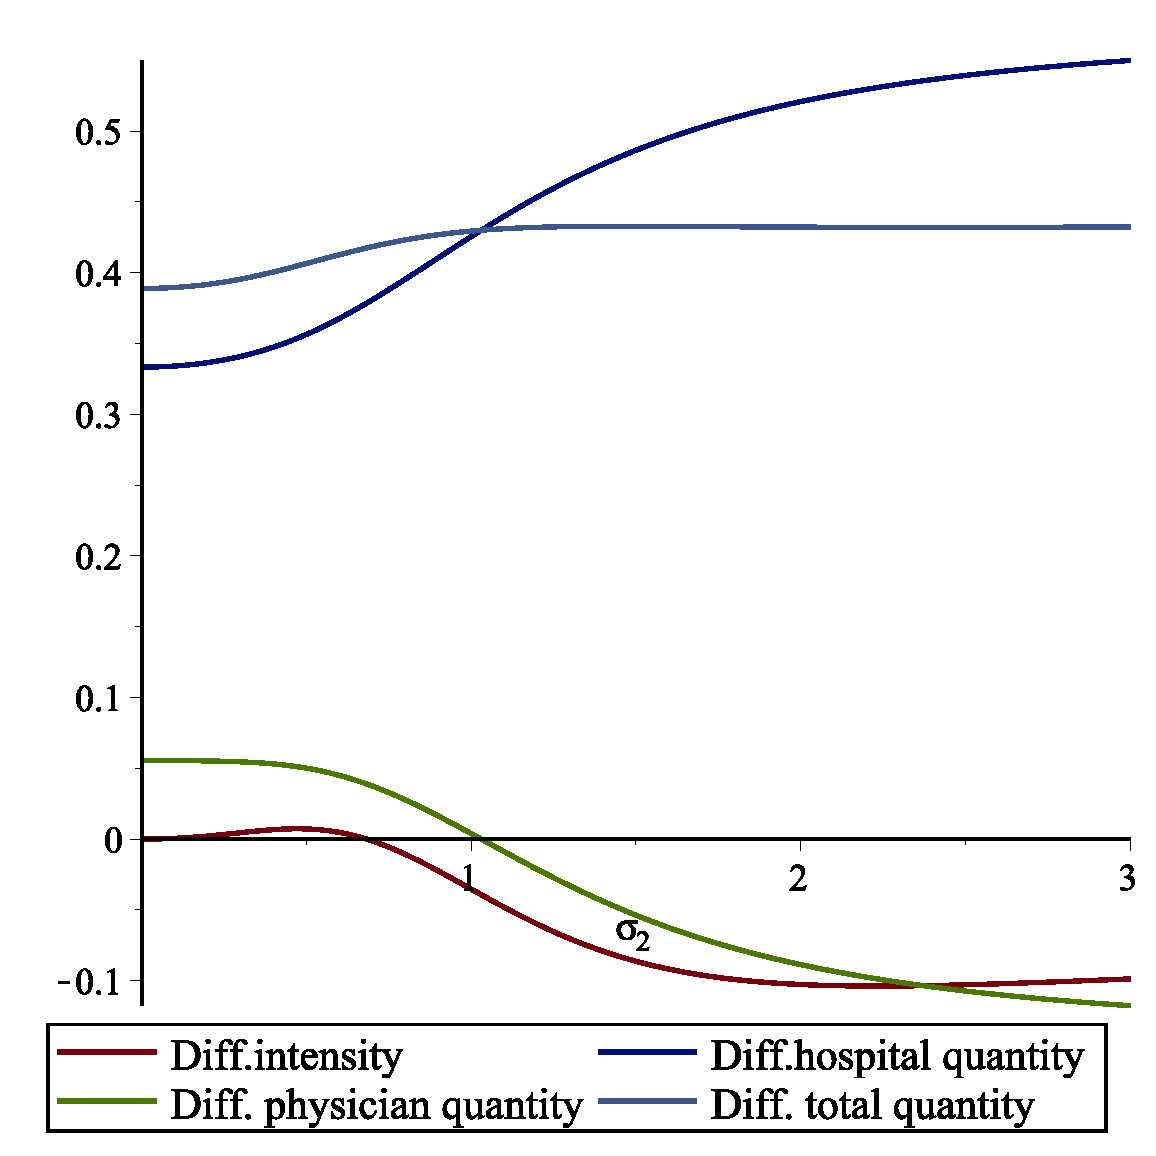
\includegraphics[width=8cm]{gr9-eps-converted-to.pdf}\\
  \caption{Diferencial de esfuerzos cuando aumenta $\sigma_2$ y las tareas son complementarias imperfectas ($\psi_{12}=-0.5$).}\label{fig11}
\end{figure}

Puede ser interesante comprobar en qué medida esta variación en el desempeño depende de la interacción entre tareas. La Figura \ref{fig11} representa los mismos resultados en diferencias de esfuerzo para tareas complementarias en la función de costes del médico. El hallazgo más destacable es que ahora se invierten los efectos iniciales sobre los esfuerzos del hospital y del médico en cantidad (el esfuerzo del médico disminuye y el del hospital aumenta en la estructura descentralizada) y, cuando $\sigma_2$ se vuelve ligeramente mayor que $\sigma_1$, el esfuerzo del médico sobre cantidad empieza a ser mayor en la estructura centralizada que en la descentralizada\footnote{Combinando este resultado con el cambio de efectos sobre las cantidades de los agentes, podemos ver que cuando $\sigma_1=0$ (medición perfecta de la cantidad), la cantidad es la misma en ambas configuraciones organizativas pero la intensidad es siempre mayor en la centralizada.}.

\section{Conclusiones}
En las páginas anteriores hemos tratado de caracterizar los rasgos principales de un modelo de provisión sanitaria en una configuración de múltiples agentes y múltiples outputs. Para ello hemos subrayado la relevancia de la información y de la estructura organizativa, así como los vínculos entre ambas. El propósito es obtener algunos resultados relevantes en términos de potencia óptima de los incentivos y de los esfuerzos ejercidos por los agentes. La restricción informativa considerada es de tipo riesgo moral tanto en los gestores hospitalarios como en los médicos. La principal cuestión de fondo a analizar es cómo la introducción de incentivos en la financiación de los hospitales tiene consecuencias distintas sobre el output dependiendo de la estructura organizativa vigente.

En un caso de referencia con información simétrica, hemos mostrado que el principal utiliza pagos de suma fija como soluciones de primer \emph{best} y mantiene a los agentes en sus utilidades de reserva. No se incluyen incentivos en el contrato óptimo. Además, médico y hospital igualan costes marginales en la producción de cantidad, y la tasa marginal de sustitución para el principal entre cantidad e intensidad debe ser igual a la tasa marginal de transformación entre tareas. Una de las implicaciones de la solución de primer \emph{best} es la relación directa entre el grado de altruismo del agente y el nivel de esfuerzo requerido.

Una vez establecido el caso de referencia, hemos pasado a estudiar el caso de acciones ocultas y riesgo moral bajo dos estructuras organizativas: una contratación centralizada (el principal trata simultáneamente con hospital y médicos) y una descentralizada (el financiador solo contrata servicios con el hospital y el hospital diseña de forma autónoma el contrato de los servicios médicos). La característica principal de la especificación del modelo es que, mientras el médico ejerce esfuerzo en las dos dimensiones (siendo estas independientes, complementarias o sustitutivas en la función de costes), el hospital solo toma decisiones sobre la cantidad de pacientes a tratar. Para derivar soluciones en forma cerrada, especificamos en consecuencia funciones de utilidad tipo CARA para los agentes, desempeños normalmente distribuidos y esquemas lineales de incentivos. El resultado general en la literatura muestra \emph{complementariedad de incentivos} cuando existen problemas de sustitución de esfuerzo\footnote{Véase \cite{Bolton05}, página 222.}. Este resultado, sin embargo, debe matizarse en nuestro modelo, ya que solo se da en la estructura descentralizada. Cuando el principal contrata cantidad tanto del hospital como del médico, la complementariedad de incentivos solo se aplica al contrato del médico, mientras que la potencia de los incentivos del hospital permanece constante e independiente de la sustitución de esfuerzos. De alguna manera, al dar autonomía al hospital conseguimos que internalice el problema de sustitución de esfuerzo y, por tanto, el principal tiene que tenerlo en cuenta en el esquema de incentivos del hospital derivado de una configuración de inducción hacia atrás.

Más interesante aún, estudiamos cómo los parámetros de incentivos de los agentes varían en los dos entornos organizativos y cómo responden a ello los niveles finales de output.
Tanto en las estructuras centralizadas como en las descentralizadas, la potencia óptima de los incentivos no depende del componente altruista o vocacional de los agentes. En la estructura centralizada los incentivos son independientes entre agentes, mientras que en la descentralizada están conectados por construcción.

Bajo una organización centralizada (la más común en el sistema hospitalario español) mostramos cómo distintos mecanismos de financiación se comportan en términos de los esfuerzos alcanzados. Como cabía esperar, la ausencia de incentivos da lugar a menores niveles de output debido a las asimetrías de información entre principal y agentes que no se tienen en cuenta.

Para el caso especial más tratable de tareas independientes en la función de costes del médico, una organización descentralizada induce mayor esfuerzo por parte del hospital y menor esfuerzo en intensidad por parte del médico que la contratación centralizada. En este escenario, si el coste marginal en cantidad del hospital es suficientemente mayor que el del médico, podríamos obtener un mejor desempeño tanto en la producción de cantidad como en la de intensidad dentro de la estructura centralizada.

Posteriormente hemos tratado de derivar algunos resultados generalizables simulando la variación en los esquemas de incentivos y en el diferencial de desempeño para ciertos valores dados de los principales parámetros fundamentales (componentes altruistas, grado de aversión al riesgo de los agentes y tecnologías de costes). Nuestro objetivo principal es ilustrar gráficamente estas simulaciones para dos cambios distintos en el entorno interactivo. Primero exploramos el problema de sustitución de esfuerzo y luego el nivel de aleatoriedad en el output bidimensional.

Respecto del grado de complementariedad o sustitución, los principales hallazgos pueden resumirse así:

\begin{itemize}
  \item Los incentivos al hospital no dependen del grado de complementariedad/sustitución entre los esfuerzos del médico en el caso centralizado. Pero sí lo hacen en un escenario descentralizado (podemos llamar a esto una especie de \emph{potencia secuencialmente inducida de los incentivos} al hospital).
  \item Las estructuras descentralizadas crean un sesgo hacia la contratación de cantidad (excepto en el caso de sustitución perfecta).
  \item Bajo tareas sustitutivas perfectas, la contratación centralizada óptima no implica incentivos para el esfuerzo del médico (salarios fijos), mientras que los incentivos permanecen positivos (y simétricos entre tareas) en un escenario descentralizado. Este resultado proporciona un vínculo teórico entre estructura organizativa y potencia de los incentivos bajo una interacción de tipo riesgo moral.
  \item Cuando la cantidad se mide perfectamente, ambas estructuras alcanzan niveles de primer \emph{best}, mientras que la intensidad es mayor en el entorno centralizado. Cuando no hay variación aleatoria en la dimensión de intensidad, ambas estructuras, de nuevo, degeneran en el caso de información plenamente simétrica, pero ahora la cantidad es mayor en el escenario descentralizado.
\end{itemize}

Cuando la principal fuente de variación está en la varianza de la medición del output, los resultados más relevantes que obtenemos del modelo son:
\begin{itemize}
  \item La complementariedad de incentivos se aplica en ambas estructuras para aumentos relativamente bajos del ruido\footnote{Excepto, trivialmente, para el incentivo del hospital sobre cantidad en la estructura de contratación separada.}. Asintóticamente, sin embargo, esta complementariedad tiende a desaparecer.
  \item Cuando la cantidad se mide de forma cada vez más imprecisa, mientras las tareas sean sustitutivas, el desempeño del hospital tiende a converger en ambas estructuras, pero el desempeño del médico es mayor en la estructura descentralizada. Si, por el contrario, las tareas son complementarias, entonces ambos desempeños del médico son mayores en el entorno centralizado. \emph{La fuente de la asimetría de información, por tanto, tiene una recomendación distinta en términos de diseño organizativo dependiendo de la interacción tecnológica entre dimensiones del output.}
  \item Cuando la intensidad es la tarea que se vuelve más ruidosa de evaluar y es sustitutiva de la cantidad, el patrón del desempeño total varía. La cantidad total permanece constante independientemente del ruido en intensidad y es mayor en una estructura descentralizada, mientras que el diferencial de intensidad crece hasta un determinado nivel de incertidumbre y luego permanece constante favoreciendo a la contratación centralizada.
  \item Cuando las tareas son complementarias, niveles bajos de ruido en intensidad favorecen a la estructura descentralizada (tanto en cantidad como incluso en intensidad). A medida que aumenta la imprecisión, los desempeños de los médicos pasan a favorecer a una estructura centralizada, compensando completamente la ventaja de la descentralizada en el esfuerzo hospitalario.
\end{itemize}

En suma, bajo riesgo moral y múltiples outputs, la estructura organizativa interactúa de formas complejas con la potencia óptima de los incentivos que debe utilizarse. En general, la intensidad es mayor en las estructuras centralizadas y la cantidad total en las descentralizadas, pero este resultado general, que debe confirmarse empíricamente, debe matizarse dependiendo de la interacción tecnológica entre tareas y del grado de incertidumbre de las medidas del output.

Los principales hallazgos de nuestro ejercicio teórico podrían traducirse en contrastes empíricos operativos que comparen, por ejemplo, las distintas puntuaciones de eficiencia de hospitales públicos o sin ánimo de lucro con las de hospitales con fines de lucro. O podríamos, eventualmente, contrastar la interacción de distintos mecanismos de pago (incentivos de baja potencia frente a incentivos de alta potencia) en diferentes arreglos organizativos. La aplicación empírica del modelo podría abordarse mediante un análisis de frontera estocástica para los datos de panel de la red hospitalaria nacional española.

\newpage
\bibliographystyle{apalike}
\bibliography{agencia}
\end{document}







